% Options for packages loaded elsewhere
\PassOptionsToPackage{unicode}{hyperref}
\PassOptionsToPackage{hyphens}{url}
%
\documentclass[
]{article}
\usepackage{amsmath,amssymb}
\usepackage{lmodern}
\usepackage{ifxetex,ifluatex}
\ifnum 0\ifxetex 1\fi\ifluatex 1\fi=0 % if pdftex
  \usepackage[T1]{fontenc}
  \usepackage[utf8]{inputenc}
  \usepackage{textcomp} % provide euro and other symbols
\else % if luatex or xetex
  \usepackage{unicode-math}
  \defaultfontfeatures{Scale=MatchLowercase}
  \defaultfontfeatures[\rmfamily]{Ligatures=TeX,Scale=1}
\fi
% Use upquote if available, for straight quotes in verbatim environments
\IfFileExists{upquote.sty}{\usepackage{upquote}}{}
\IfFileExists{microtype.sty}{% use microtype if available
  \usepackage[]{microtype}
  \UseMicrotypeSet[protrusion]{basicmath} % disable protrusion for tt fonts
}{}
\makeatletter
\@ifundefined{KOMAClassName}{% if non-KOMA class
  \IfFileExists{parskip.sty}{%
    \usepackage{parskip}
  }{% else
    \setlength{\parindent}{0pt}
    \setlength{\parskip}{6pt plus 2pt minus 1pt}}
}{% if KOMA class
  \KOMAoptions{parskip=half}}
\makeatother
\usepackage{xcolor}
\IfFileExists{xurl.sty}{\usepackage{xurl}}{} % add URL line breaks if available
\IfFileExists{bookmark.sty}{\usepackage{bookmark}}{\usepackage{hyperref}}
\hypersetup{
  pdftitle={Supplementary Material},
  pdfauthor={Arthur M. Albuquerque},
  hidelinks,
  pdfcreator={LaTeX via pandoc}}
\urlstyle{same} % disable monospaced font for URLs
\usepackage[margin=1in]{geometry}
\usepackage{graphicx}
\makeatletter
\def\maxwidth{\ifdim\Gin@nat@width>\linewidth\linewidth\else\Gin@nat@width\fi}
\def\maxheight{\ifdim\Gin@nat@height>\textheight\textheight\else\Gin@nat@height\fi}
\makeatother
% Scale images if necessary, so that they will not overflow the page
% margins by default, and it is still possible to overwrite the defaults
% using explicit options in \includegraphics[width, height, ...]{}
\setkeys{Gin}{width=\maxwidth,height=\maxheight,keepaspectratio}
% Set default figure placement to htbp
\makeatletter
\def\fps@figure{htbp}
\makeatother
\setlength{\emergencystretch}{3em} % prevent overfull lines
\providecommand{\tightlist}{%
  \setlength{\itemsep}{0pt}\setlength{\parskip}{0pt}}
\setcounter{secnumdepth}{-\maxdimen} % remove section numbering
\newcommand*\fillCircle{\tikz{\filldraw (0,0) circle (3pt)}}
\newcommand*\emptyCircle{\tikz{\draw (0,0) circle (3pt)}}
\usepackage{tikz}
\usepackage{booktabs}
\usepackage{longtable}
\usepackage{array}
\usepackage{multirow}
\usepackage{wrapfig}
\usepackage{float}
\usepackage{colortbl}
\usepackage{pdflscape}
\usepackage{tabu}
\usepackage{threeparttable}
\usepackage{threeparttablex}
\usepackage[normalem]{ulem}
\usepackage{makecell}
\usepackage{xcolor}
\ifluatex
  \usepackage{selnolig}  % disable illegal ligatures
\fi

\title{Supplementary Material}
\author{Arthur M. Albuquerque}
\date{June 03, 2021}

\begin{document}
\maketitle

{
\setcounter{tocdepth}{3}
\tableofcontents
}
\hypertarget{data-extraction}{%
\section{Data extraction}\label{data-extraction}}

In this section, we will elaborate the details underlying our data
extraction process.

We pre-registered our protocol in the OpenScienceFramework
(\url{https://osf.io/cytq8/}). In brief, we extracted summary data from
randomized controlled trials (RCT) included in a living systematic
review on Cochrane. We accessed each individual RCT manuscript to
extract data. We contacted the authors by e-mail to obtain relevant data
not available in the manuscript. However, we did not have success to
obtain any extra information by e-mail.

The tables below show what studies were included and excluded. We will
also show the direct source (Figure/Table) of the extracted data in each
RCT. Lastly, we show relevant notes about details from each study and
why we did not extract data from certain RCTs that were included in the
living systematic.

The diagram below show the workflow regarding studies that were used to
create prior distributions.

\begin{center}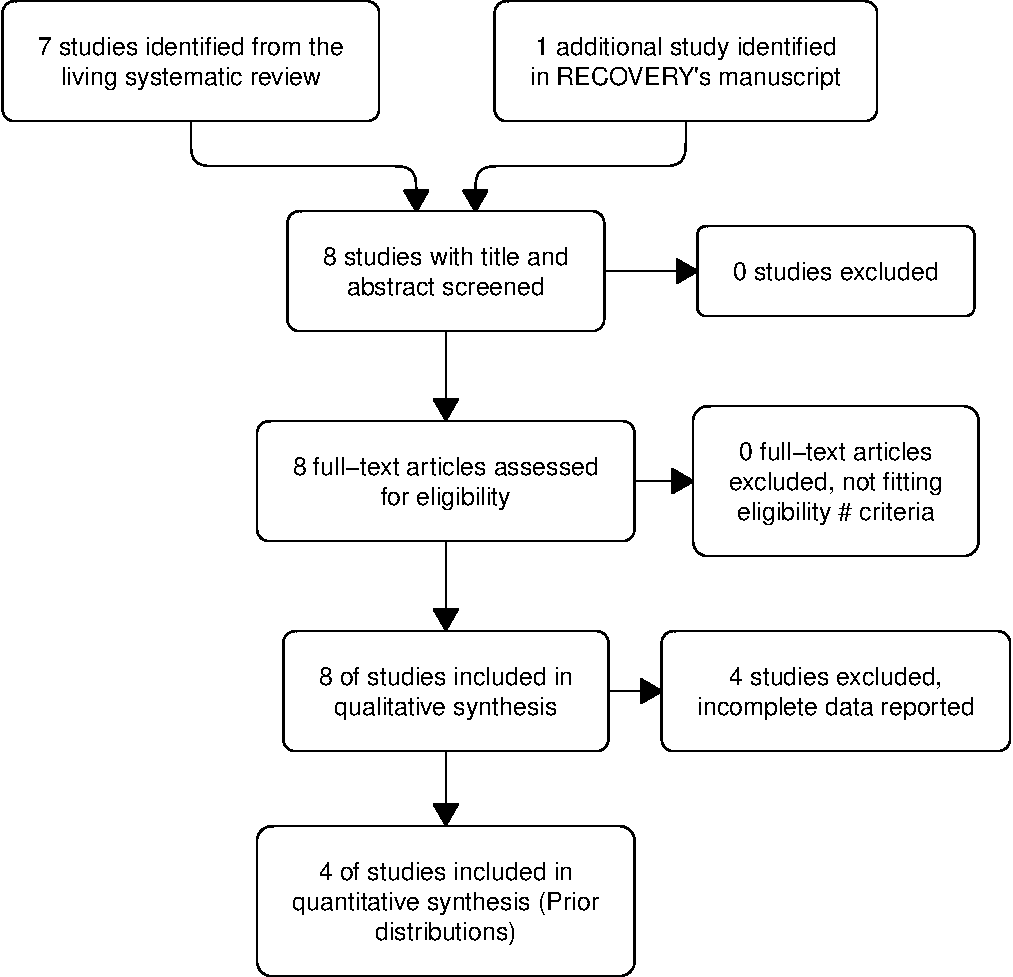
\includegraphics[width=0.7\linewidth]{supplementary_files/figure-latex/unnamed-chunk-3-1} \end{center}

\newpage

\begin{landscape}\begin{table}

\caption{\label{tab:unnamed-chunk-4}Included studies for the mortality outcome}
\centering
\begin{tabular}[t]{>{\centering\arraybackslash}p{18em}>{\centering\arraybackslash}p{6em}>{\centering\arraybackslash}p{40em}}
\toprule
Study & Source & Notes\\
\midrule
\addlinespace[0.3em]
\multicolumn{3}{l}{\textbf{Not using corticosteroids}}\\
\hspace{1em}\cellcolor{gray!6}{RECOVERY} & \cellcolor{gray!6}{Figure 3} & \cellcolor{gray!6}{"Use of corticosteroids" \vphantom{1} section}\\
\hspace{1em}COVACTA & Table S10 & Ordinal category 7 means \vphantom{1} death.\\
\hspace{1em}\cellcolor{gray!6}{REMAP-CAP} & \cellcolor{gray!6}{Figure 9} & \cellcolor{gray!6}{Full explanation in another section of this supplementary \vphantom{1} material}\\
\addlinespace[0.3em]
\multicolumn{3}{l}{\textbf{Using corticosteroids}}\\
\hspace{1em}RECOVERY & Figure 3 & "Use of corticosteroids" section\\
\hspace{1em}\cellcolor{gray!6}{COVACTA} & \cellcolor{gray!6}{Table S10} & \cellcolor{gray!6}{Ordinal category 7 means death.}\\
\hspace{1em}REMAP-CAP & Figure 9 & Full explanation in another section of this supplementary material\\
\addlinespace[0.3em]
\multicolumn{3}{l}{\textbf{Simple oxygen only}}\\
\hspace{1em}\cellcolor{gray!6}{RECOVERY} & \cellcolor{gray!6}{Figure 3} & \cellcolor{gray!6}{"Respiratory support at randomisation" \vphantom{2} section}\\
\hspace{1em}COVACTA & Figure 2 & Ordinal category 3 means "non–ICU hospitalization with supplemental oxygen". Thus, Category 3 at baseline equals to the "simple oxygen only" subgroup. Ordinal Category 7 means death.\\
\hspace{1em}\cellcolor{gray!6}{CORIMUNO-19} & \cellcolor{gray!6}{Table 2} & \cellcolor{gray!6}{This study only included patients "...receiving at least 3L/min oxygen (O2) but without high-flow oxygen (HFO)...". Thus, we included all data available.}\\
\addlinespace[0.3em]
\multicolumn{3}{l}{\textbf{Non-invasive ventilation}}\\
\hspace{1em}RECOVERY & Figure 3 & "Respiratory support at randomisation" \vphantom{1} section\\
\hspace{1em}\cellcolor{gray!6}{COVACTA} & \cellcolor{gray!6}{Figure 2} & \cellcolor{gray!6}{Ordinal category 4 means "ICU or non–ICU hospitalization with noninvasive ventilation or high-flow oxygen". Thus, Category 4 at baseline equals to the "non-invasive ventilation" subgroup. Ordinal Category 7 means death.}\\
\hspace{1em}REMAP-CAP & Table S7 & "Progression to invasive mechanical ventilation, ECMO or death, restricted to those not intubated at baseline" section\\
\hspace{1em}\cellcolor{gray!6}{Salvarini} & \cellcolor{gray!6}{Table 2} & \cellcolor{gray!6}{This study only included patients "Patients at enrollment were allowed to receive oxygen therapy with Venturi mask or high-flow nasal cannula with recorded and preset FIO2...". Thus, we included all data available.}\\
\addlinespace[0.3em]
\multicolumn{3}{l}{\textbf{Invasive mechanical ventilation}}\\
\hspace{1em}RECOVERY & Figure 3 & "Respiratory support at randomisation" section\\
\hspace{1em}\cellcolor{gray!6}{COVACTA} & \cellcolor{gray!6}{Figure 2} & \cellcolor{gray!6}{Ordinal category 5 means "ICU hospitalization with mechanical ventilation" and category 6 means "ICU hospitalization with extracorporeal membrane oxygenation or mechanical ventilation and additional organ support". Thus, both categories combined equals to the "invasive mechanical ventilation" subgroup. Ordinal Category 7 means death.}\\
\hspace{1em}REMAP-CAP & Table 2 and Table S7 & Table S7 shows how many patients that were free of IMV at baseline died (53 and 82) and their sample size (242 + 273). Table 2 shows total number of deaths (98 and 142) and total sample size (350 + 397). Thus, we subtracted values between tables to get how many patients on IMV at baseline died and sample size.\\
\bottomrule
\end{tabular}
\end{table}
\end{landscape}

\begin{landscape}\begin{table}

\caption{\label{tab:unnamed-chunk-5}Included studies for the hospital discharge outcome}
\centering
\begin{tabular}[t]{>{\centering\arraybackslash}p{18em}>{\centering\arraybackslash}p{6em}>{\centering\arraybackslash}p{40em}}
\toprule
Study & Source & Notes\\
\midrule
\addlinespace[0.3em]
\multicolumn{3}{l}{\textbf{Not using corticosteroids}}\\
\hspace{1em}\cellcolor{gray!6}{RECOVERY} & \cellcolor{gray!6}{Webfigure 1} & \cellcolor{gray!6}{"Use of corticosteroids" \vphantom{1} section}\\
\hspace{1em}COVACTA & Table S10 & Ordinal category 1 means "discharged or ready for \vphantom{1} discharge"\\
\addlinespace[0.3em]
\multicolumn{3}{l}{\textbf{Using corticosteroids}}\\
\hspace{1em}\cellcolor{gray!6}{RECOVERY} & \cellcolor{gray!6}{Webfigure 1} & \cellcolor{gray!6}{"Use of corticosteroids" section}\\
\hspace{1em}COVACTA & Table S10 & Ordinal category 1 means "discharged or ready for discharge"\\
\addlinespace[0.3em]
\multicolumn{3}{l}{\textbf{Simple oxygen only}}\\
\hspace{1em}\cellcolor{gray!6}{RECOVERY} & \cellcolor{gray!6}{Webfigure 1} & \cellcolor{gray!6}{"Respiratory support at randomisation" \vphantom{2} section}\\
\hspace{1em}COVACTA & Figure 2 & Ordinal category 3 means "non–ICU hospitalization with supplemental oxygen". Thus, Category 3 at baseline equals to the "simple oxygen only" subgroup. Ordinal Category 7 means "discharged or ready for discharge".\\
\hspace{1em}\cellcolor{gray!6}{CORIMUNO-19} & \cellcolor{gray!6}{eTable 9} & \cellcolor{gray!6}{This study only included patients "...receiving at least 3L/min oxygen (O2) but without high-flow oxygen (HFO)...". Thus, we included all data available.}\\
\addlinespace[0.3em]
\multicolumn{3}{l}{\textbf{Non-invasive ventilation}}\\
\hspace{1em}RECOVERY & Webfigure 1 & "Respiratory support at randomisation" \vphantom{1} section\\
\hspace{1em}\cellcolor{gray!6}{COVACTA} & \cellcolor{gray!6}{Figure 2} & \cellcolor{gray!6}{Ordinal category 4 means "ICU or non–ICU hospitalization with noninvasive ventilation or high-flow oxygen". Thus, Category 4 at baseline equals to the "non-invasive ventilation" subgroup. Ordinal Category 7 means "discharged or ready for discharge".}\\
\hspace{1em}Salvarini & Table 2 & This study only included patients "Patients at enrollment were allowed to receive oxygen therapy with Venturi mask or high-flow nasal cannula with recorded and preset FIO2...". Thus, we included all data available.\\
\addlinespace[0.3em]
\multicolumn{3}{l}{\textbf{Invasive mechanical ventilation}}\\
\hspace{1em}\cellcolor{gray!6}{RECOVERY} & \cellcolor{gray!6}{Webfigure 1} & \cellcolor{gray!6}{"Respiratory support at randomisation" section}\\
\hspace{1em}COVACTA & Figure 2 & Ordinal category 5 means "ICU hospitalization with mechanical ventilation" and category 6 means "ICU hospitalization with extracorporeal membrane oxygenation or mechanical ventilation and additional organ support". Thus, both categories combined equals to the "invasive mechanical ventilation" subgroup. Ordinal Category 7 means "discharged or ready for discharge".\\
\bottomrule
\end{tabular}
\end{table}
\end{landscape}

\begin{landscape}\begin{table}

\caption{\label{tab:unnamed-chunk-6}Excluded studies for the mortality outcome}
\centering
\begin{tabular}[t]{>{\raggedright\arraybackslash}p{18em}>{\raggedright\arraybackslash}p{20em}}
\toprule
Study & Notes\\
\midrule
\addlinespace[0.3em]
\multicolumn{2}{l}{\textbf{Use of corticosteroids subgroups}}\\
\hspace{1em}\cellcolor{gray!6}{TOCIBRAS} & \cellcolor{gray!6}{Not possible to extract data per \vphantom{1} subgroup}\\
\hspace{1em}Stone & Not possible to extract data per \vphantom{1} subgroup\\
\hspace{1em}\cellcolor{gray!6}{EMPACTA} & \cellcolor{gray!6}{Not possible to extract data per \vphantom{1} subgroup}\\
\hspace{1em}COVINTOC & Not reported\\
\addlinespace[0.3em]
\multicolumn{2}{l}{\textbf{Respiratory support subgroups}}\\
\hspace{1em}\cellcolor{gray!6}{TOCIBRAS} & \cellcolor{gray!6}{Not possible to extract data per subgroup}\\
\hspace{1em}Stone & Not possible to extract data per subgroup\\
\hspace{1em}\cellcolor{gray!6}{EMPACTA} & \cellcolor{gray!6}{Not possible to extract data per subgroup}\\
\hspace{1em}COVINTOC & Not possible to extract data per subgroup\\
\bottomrule
\end{tabular}
\end{table}
\end{landscape}

\begin{landscape}\begin{table}

\caption{\label{tab:unnamed-chunk-7}Excluded studies for the hospital discharge outcome}
\centering
\begin{tabular}[t]{>{\raggedright\arraybackslash}p{18em}>{\raggedright\arraybackslash}p{20em}}
\toprule
Study & Notes\\
\midrule
\addlinespace[0.3em]
\multicolumn{2}{l}{\textbf{Use of corticosteroids subgroups}}\\
\hspace{1em}\cellcolor{gray!6}{REMAP-CAP} & \cellcolor{gray!6}{Not reported}\\
\hspace{1em}TOCIBRAS & Not possible to extract data per \vphantom{1} subgroup\\
\hspace{1em}\cellcolor{gray!6}{Stone} & \cellcolor{gray!6}{Not possible to extract data per \vphantom{1} subgroup}\\
\hspace{1em}EMPACTA & Not possible to extract data per \vphantom{1} subgroup\\
\hspace{1em}\cellcolor{gray!6}{COVINTOC} & \cellcolor{gray!6}{Not \vphantom{1} reported}\\
\addlinespace[0.3em]
\multicolumn{2}{l}{\textbf{Respiratory support subgroups}}\\
\hspace{1em}REMAP-CAP & Not possible to extract data per subgroup\\
\hspace{1em}\cellcolor{gray!6}{TOCIBRAS} & \cellcolor{gray!6}{Not possible to extract data per subgroup}\\
\hspace{1em}Stone & Not possible to extract data per subgroup\\
\hspace{1em}\cellcolor{gray!6}{EMPACTA} & \cellcolor{gray!6}{Not possible to extract data per subgroup}\\
\hspace{1em}COVINTOC & Not reported\\
\bottomrule
\end{tabular}
\end{table}
\end{landscape}

\newpage

As mentioned in the tables above, we will now discuss further details
about data on the use of corticosteroids subgroups from REMAP-CAP.

The relevant data from these subgroups are shown in Figure 9 in their
supplementary material. Unfortunately, the authors do not provide the
raw number of events per subgroup. Instead, the data is displayed
visually in stacked bars. Thus, we used the
\href{https://cran.r-project.org/web/packages/juicr/index.html}{\{juicr\}
package} to extract data directly from Figure 9. The raw data and
extraction report generated by \{juicr\} can be found in this project's
\href{https://github.com/arthur-albuquerque/tocilizumab_reanalysis/tree/master/final_analyses/data}{GitHub
repository}.

Of note, REMAP-CAP was a three-arm randomized controlled trial that
tested tocilizumab and sarilumab (both are IL-6 antagonists) vs.~usual
care. The authors only provided pooled data from these IL-6 antagonists
vs.~usual care in Figure 9. Thus, we decided to perform sensitivity
analyses with this data to dampen the influence of sarilumab in final
results.

We created evidence-based priors for these subgroups using data from
REMAP-CAP with different weights: 100\%, 75\% and 50\%. This approach
implies that the numbers of events and sample sizes from REMAP-CAP were
multiplied by 1, 0.75 or 0.5, respectively.

As mentioned in the Methods section, we pooled data from similar studies
with a random-effect meta-analysis using a restricted maximum-likelihood
estimator to create evidence-based priors. We will now display
evidence-based prior distributions for both ``Not using
corticosteroids'' and ``Using corticosteroids'' subgroups that were
generated with different weights on REMAP-CAP. Top panels regards ``Not
using corticosteroids'' and the bottom panels ``Using corticosteroids''.
We show these distributions in both log-odds ratio and odds ratio scales
to ease interpretation.

\begin{center}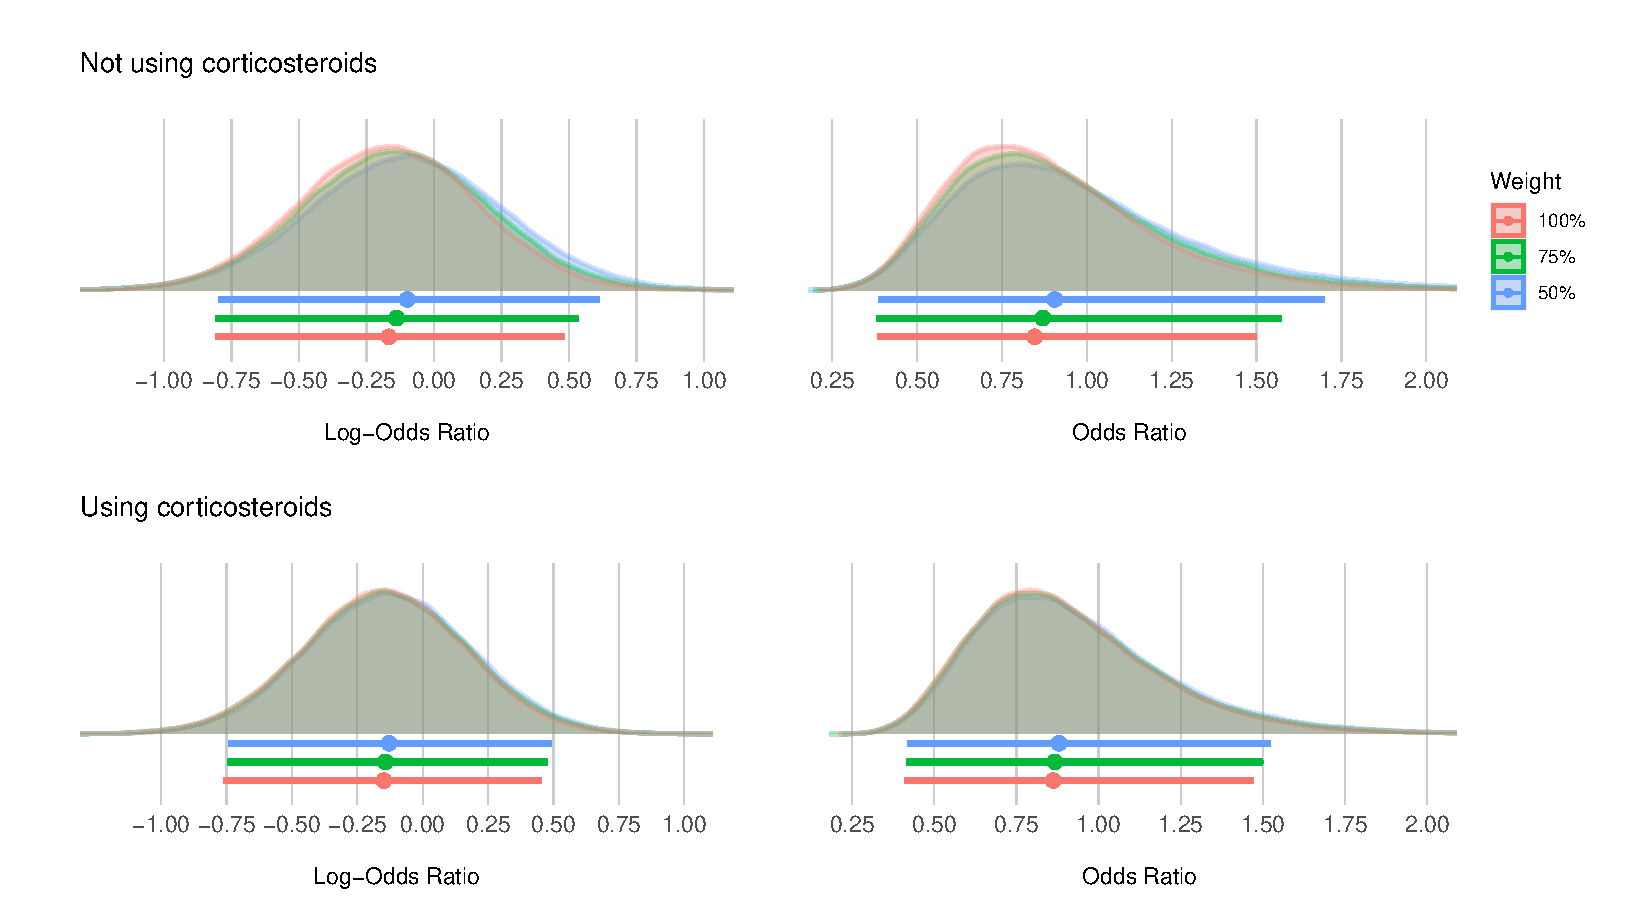
\includegraphics[width=1.1\linewidth]{/Users/arthur/Coding/projects/tocilizumab_reanalysis/final_analyses/output/plots/appendix/weight_remap_cap_corticosteroids} \end{center}

Point estimates depict the median and interval bars depict the 95\%
highest density interval.

Because prior distributions are notably similar regardless of the weight
used, we have decided to only use the ones with 100\% weight for our
analyses.

\newpage

\hypertarget{overall-characteristics}{%
\section{Overall characteristics}\label{overall-characteristics}}

\begin{table}[!h]

\caption{\label{tab:unnamed-chunk-10}Overall characteristics of included studies}
\centering
\begin{tabular}[t]{>{\raggedright\arraybackslash}p{15em}l}
\toprule
Study Characteristic &  \\
\midrule
\addlinespace[0.3em]
\multicolumn{2}{l}{\textbf{RECOVERY}}\\
\hspace{1em}\cellcolor{gray!6}{Year} & \cellcolor{gray!6}{2021}\\
\hspace{1em}Trial design & Open-label\\
\hspace{1em}\cellcolor{gray!6}{Follow-up period (days)} & \cellcolor{gray!6}{28}\\
\hspace{1em}Control treatment & Standard of care\\
\addlinespace[0.3em]
\multicolumn{2}{l}{\textbf{COVACTA}}\\
\hspace{1em}\cellcolor{gray!6}{Year} & \cellcolor{gray!6}{2021}\\
\hspace{1em}Trial design & Double-blinded\\
\hspace{1em}\cellcolor{gray!6}{Follow-up period (days)} & \cellcolor{gray!6}{28}\\
\hspace{1em}Control treatment & Placebo\\
\addlinespace[0.3em]
\multicolumn{2}{l}{\textbf{REMAP-CAP}}\\
\hspace{1em}\cellcolor{gray!6}{Year} & \cellcolor{gray!6}{2021}\\
\hspace{1em}Trial design & Open-label\\
\hspace{1em}\cellcolor{gray!6}{Follow-up period (days)} & \cellcolor{gray!6}{21}\\
\hspace{1em}Control treatment & Standard of care\\
\addlinespace[0.3em]
\multicolumn{2}{l}{\textbf{CORIMUNO-19}}\\
\hspace{1em}\cellcolor{gray!6}{Year} & \cellcolor{gray!6}{2020}\\
\hspace{1em}Trial design & Open-label\\
\hspace{1em}\cellcolor{gray!6}{Follow-up period (days)} & \cellcolor{gray!6}{28}\\
\hspace{1em}Control treatment & Standard of care\\
\addlinespace[0.3em]
\multicolumn{2}{l}{\textbf{Salvarini}}\\
\hspace{1em}\cellcolor{gray!6}{Year} & \cellcolor{gray!6}{2020}\\
\hspace{1em}Trial design & Open-label\\
\hspace{1em}\cellcolor{gray!6}{Follow-up period (days)} & \cellcolor{gray!6}{30}\\
\hspace{1em}Control treatment & Standard of care\\
\bottomrule
\end{tabular}
\end{table}

\begin{table}

\caption{\label{tab:unnamed-chunk-11}Patient characteristics of included studies (Filled circles indicate what subgroups from each trial were used for outcome analyses)}
\centering
\begin{tabular}[t]{>{\raggedright\arraybackslash}p{25em}>{\centering\arraybackslash}p{6.5em}>{\centering\arraybackslash}p{6.5em}>{\centering\arraybackslash}p{3.5em}>{\centering\arraybackslash}p{6em}}
\toprule
\multicolumn{1}{c}{ } & \multicolumn{2}{c}{Interventions} & \multicolumn{2}{c}{Outcomes} \\
\cmidrule(l{3pt}r{3pt}){2-3} \cmidrule(l{3pt}r{3pt}){4-5}
Study Characteristic & Control & Tocilizumab & Mortality & Hospital Discharge\\
\midrule
\addlinespace[0.3em]
\multicolumn{5}{l}{\textbf{RECOVERY}}\\
\hspace{1em}\cellcolor{gray!6}{Number of patients} & \cellcolor{gray!6}{2094} & \cellcolor{gray!6}{2022} & \cellcolor{gray!6}{} & \cellcolor{gray!6}{}\\
\hspace{1em}Age (SD) & 64 (14) & 63 (14) &  & \\
\hspace{1em}\cellcolor{gray!6}{Male sex (\%)} & \cellcolor{gray!6}{69} & \cellcolor{gray!6}{66} & \cellcolor{gray!6}{} & \cellcolor{gray!6}{}\\
\hspace{1em}Confirmed SARS-CoV-2 infection (\%) & 96 & 95 &  & \\
\hspace{1em}\cellcolor{gray!6}{Use of corticosteroids (\%)} & \cellcolor{gray!6}{82} & \cellcolor{gray!6}{82} & \cellcolor{gray!6}{\fillCircle} & \cellcolor{gray!6}{\fillCircle}\\
\hspace{1em}Simple oxygen only at randomisation (\%) & 45 & 46 & \fillCircle & \fillCircle\\
\hspace{1em}\cellcolor{gray!6}{Non-invasive ventilation at randomisation (\%)} & \cellcolor{gray!6}{41} & \cellcolor{gray!6}{41} & \cellcolor{gray!6}{\fillCircle} & \cellcolor{gray!6}{\fillCircle}\\
\hspace{1em}Invasive mechanical ventilation at randomisation (\%) & 14 & 13 & \fillCircle & \fillCircle\\
\addlinespace[0.3em]
\multicolumn{5}{l}{\textbf{COVACTA}}\\
\hspace{1em}\cellcolor{gray!6}{Number of patients} & \cellcolor{gray!6}{144} & \cellcolor{gray!6}{294} & \cellcolor{gray!6}{} & \cellcolor{gray!6}{}\\
\hspace{1em}Age (SD) & 61 (14) & 60 (15) &  & \\
\hspace{1em}\cellcolor{gray!6}{Male sex (\%)} & \cellcolor{gray!6}{70} & \cellcolor{gray!6}{70} & \cellcolor{gray!6}{} & \cellcolor{gray!6}{}\\
\hspace{1em}Confirmed SARS-CoV-2 infection (\%) & 100 & 100 &  \vphantom{1} & \\
\hspace{1em}\cellcolor{gray!6}{Use of corticosteroids (\%)} & \cellcolor{gray!6}{28.5} & \cellcolor{gray!6}{19} & \cellcolor{gray!6}{\fillCircle} & \cellcolor{gray!6}{\fillCircle}\\
\hspace{1em}Simple oxygen only at randomisation (\%) & 31 & 26.5 & \fillCircle & \fillCircle\\
\hspace{1em}\cellcolor{gray!6}{Non-invasive ventilation at randomisation (\%)} & \cellcolor{gray!6}{27} & \cellcolor{gray!6}{32} & \cellcolor{gray!6}{\fillCircle} & \cellcolor{gray!6}{\fillCircle}\\
\hspace{1em}Invasive mechanical ventilation at randomisation (\%) & 38 & 38 & \fillCircle & \fillCircle\\
\addlinespace[0.3em]
\multicolumn{5}{l}{\textbf{REMAP-CAP}}\\
\hspace{1em}\cellcolor{gray!6}{Number of patients} & \cellcolor{gray!6}{402} & \cellcolor{gray!6}{353} & \cellcolor{gray!6}{} & \cellcolor{gray!6}{}\\
\hspace{1em}Age (SD) & 61 (13) & 61  (12) &  & \\
\hspace{1em}\cellcolor{gray!6}{Male sex (\%)} & \cellcolor{gray!6}{70} & \cellcolor{gray!6}{74} & \cellcolor{gray!6}{} & \cellcolor{gray!6}{}\\
\hspace{1em}Confirmed SARS-CoV-2 infection (\%) & 85 & 82 &  & \\
\hspace{1em}\cellcolor{gray!6}{Use of corticosteroids (\%)} & \cellcolor{gray!6}{> 80} & \cellcolor{gray!6}{> 80} & \cellcolor{gray!6}{\fillCircle} & \cellcolor{gray!6}{\emptyCircle}\\
\hspace{1em}Simple oxygen only at randomisation (\%) & < 1 & < 1 & \emptyCircle & \emptyCircle\\
\hspace{1em}\cellcolor{gray!6}{Non-invasive ventilation at randomisation (\%)} & \cellcolor{gray!6}{69} & \cellcolor{gray!6}{71} & \cellcolor{gray!6}{\fillCircle} & \cellcolor{gray!6}{\emptyCircle}\\
\hspace{1em}Invasive mechanical ventilation at randomisation (\%) & 30 & 29 & \fillCircle & \emptyCircle\\
\addlinespace[0.3em]
\multicolumn{5}{l}{\textbf{CORIMUNO}}\\
\hspace{1em}\cellcolor{gray!6}{Number of patients} & \cellcolor{gray!6}{67} & \cellcolor{gray!6}{63} & \cellcolor{gray!6}{} & \cellcolor{gray!6}{}\\
\hspace{1em}Age (IQR) & 63 (57 - 72) & 64 (57 - 74) &  & \\
\hspace{1em}\cellcolor{gray!6}{Male sex (\%)} & \cellcolor{gray!6}{66} & \cellcolor{gray!6}{70} & \cellcolor{gray!6}{} & \cellcolor{gray!6}{}\\
\hspace{1em}Confirmed SARS-CoV-2 infection (\%) & 90 & 89 &  & \\
\hspace{1em}\cellcolor{gray!6}{Use of corticosteroids (\%)} & \cellcolor{gray!6}{61} & \cellcolor{gray!6}{33} & \cellcolor{gray!6}{\emptyCircle} & \cellcolor{gray!6}{\emptyCircle}\\
\hspace{1em}Simple oxygen only at randomisation (\%) & 100 & 100 & \fillCircle & \fillCircle\\
\hspace{1em}\cellcolor{gray!6}{Non-invasive ventilation at randomisation (\%)} & \cellcolor{gray!6}{0} & \cellcolor{gray!6}{0} & \cellcolor{gray!6}{\emptyCircle} & \cellcolor{gray!6}{\emptyCircle}\\
\hspace{1em}Invasive mechanical ventilation at randomisation (\%) & 0 & 0 & \emptyCircle & \emptyCircle\\
\addlinespace[0.3em]
\multicolumn{5}{l}{\textbf{Salvarini}}\\
\hspace{1em}\cellcolor{gray!6}{Number of patients} & \cellcolor{gray!6}{62} & \cellcolor{gray!6}{60} & \cellcolor{gray!6}{} & \cellcolor{gray!6}{}\\
\hspace{1em}Age (IQR) & 60 (54 - 69) & 61 (51 - 73) &  & \\
\hspace{1em}\cellcolor{gray!6}{Male sex (\%)} & \cellcolor{gray!6}{56} & \cellcolor{gray!6}{67} & \cellcolor{gray!6}{} & \cellcolor{gray!6}{}\\
\hspace{1em}Confirmed SARS-CoV-2 infection (\%) & 100 & 100 &  & \\
\hspace{1em}\cellcolor{gray!6}{Use of corticosteroids (\%)} & \cellcolor{gray!6}{11} & \cellcolor{gray!6}{10} & \cellcolor{gray!6}{\emptyCircle} & \cellcolor{gray!6}{\emptyCircle}\\
\hspace{1em}Simple oxygen only at randomisation (\%) & 0 & 0 & \emptyCircle & \emptyCircle\\
\hspace{1em}\cellcolor{gray!6}{Non-invasive ventilation at randomisation (\%)} & \cellcolor{gray!6}{100} & \cellcolor{gray!6}{100} & \cellcolor{gray!6}{\fillCircle} & \cellcolor{gray!6}{\fillCircle}\\
\hspace{1em}Invasive mechanical ventilation at randomisation (\%) & 0 & 0 & \emptyCircle & \emptyCircle\\
\bottomrule
\end{tabular}
\end{table}

\newpage

\hypertarget{results-mortality-outcome}{%
\section{Results: Mortality outcome}\label{results-mortality-outcome}}

\hypertarget{prior-recovery-and-posterior-distributions}{%
\subsection{Prior, RECOVERY, and Posterior
distributions}\label{prior-recovery-and-posterior-distributions}}

\hypertarget{supplementary-table-1}{%
\subsubsection{Supplementary Table 1}\label{supplementary-table-1}}

\begin{center}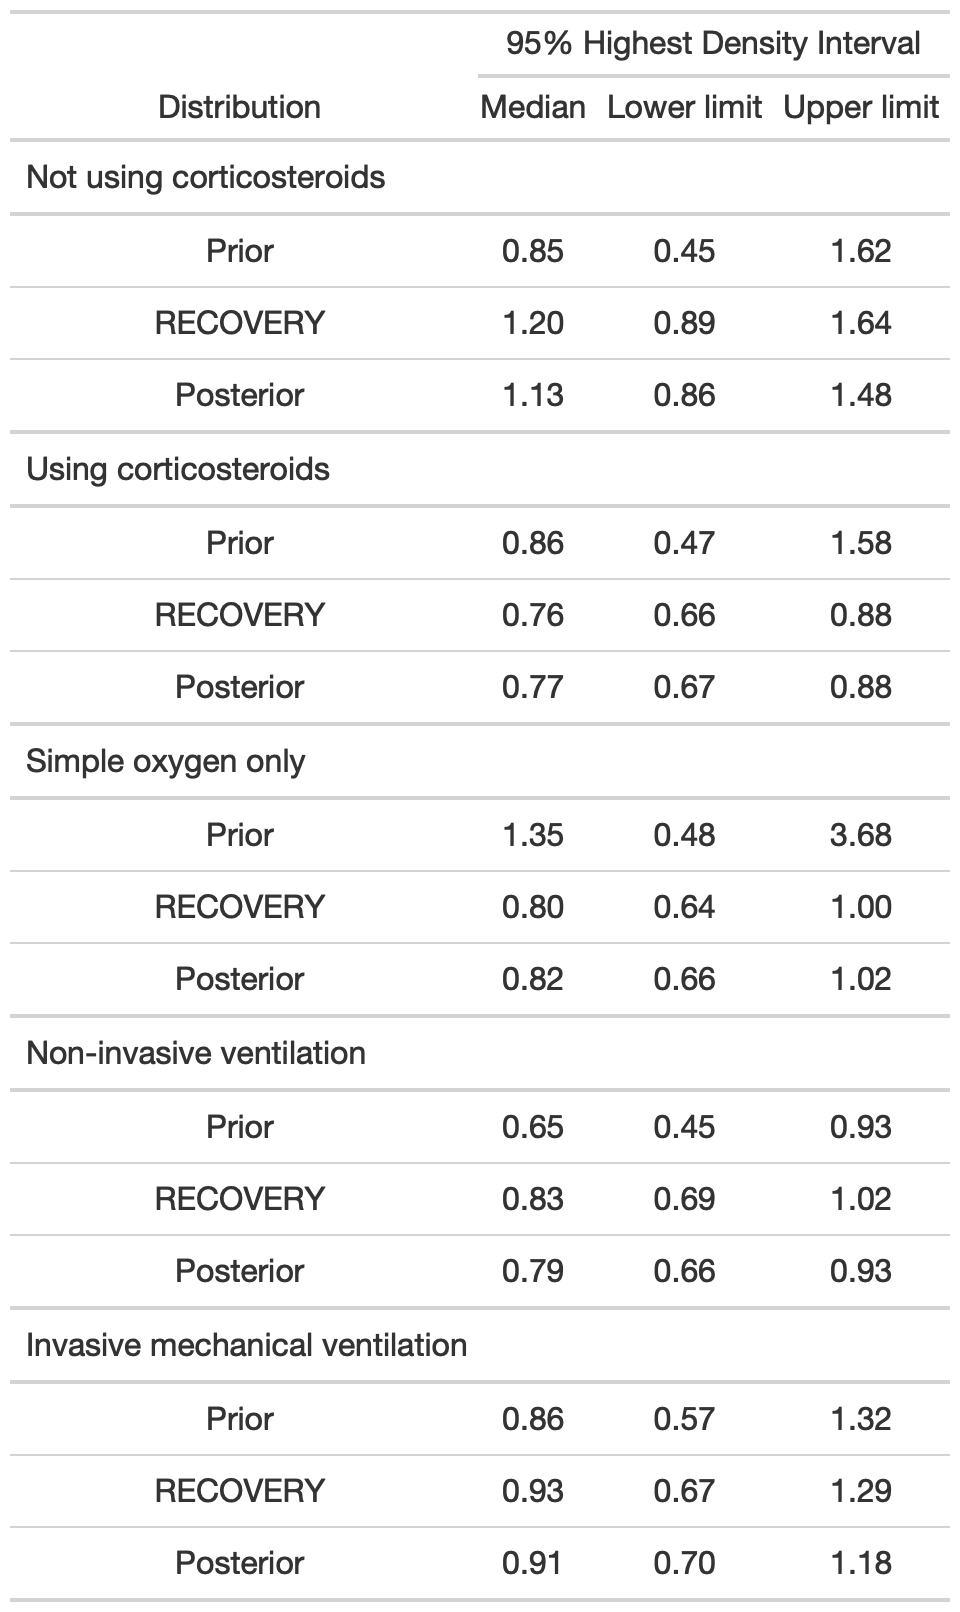
\includegraphics[width=0.6\linewidth]{/Users/arthur/Coding/projects/tocilizumab_reanalysis/final_analyses/output/plots/appendix/STable1_HDI_intervals_figure1} \end{center}

95\% highest density intervals of evidence-based prior, RECOVERY, and
posterior distributions. This table complements Figure 1.

\newpage

\hypertarget{posterior-probabilities-using-evidence-based-priors}{%
\subsection{Posterior probabilities using evidence-based
priors}\label{posterior-probabilities-using-evidence-based-priors}}

\hypertarget{supplementary-table-2}{%
\subsubsection{Supplementary Table 2}\label{supplementary-table-2}}

\begin{center}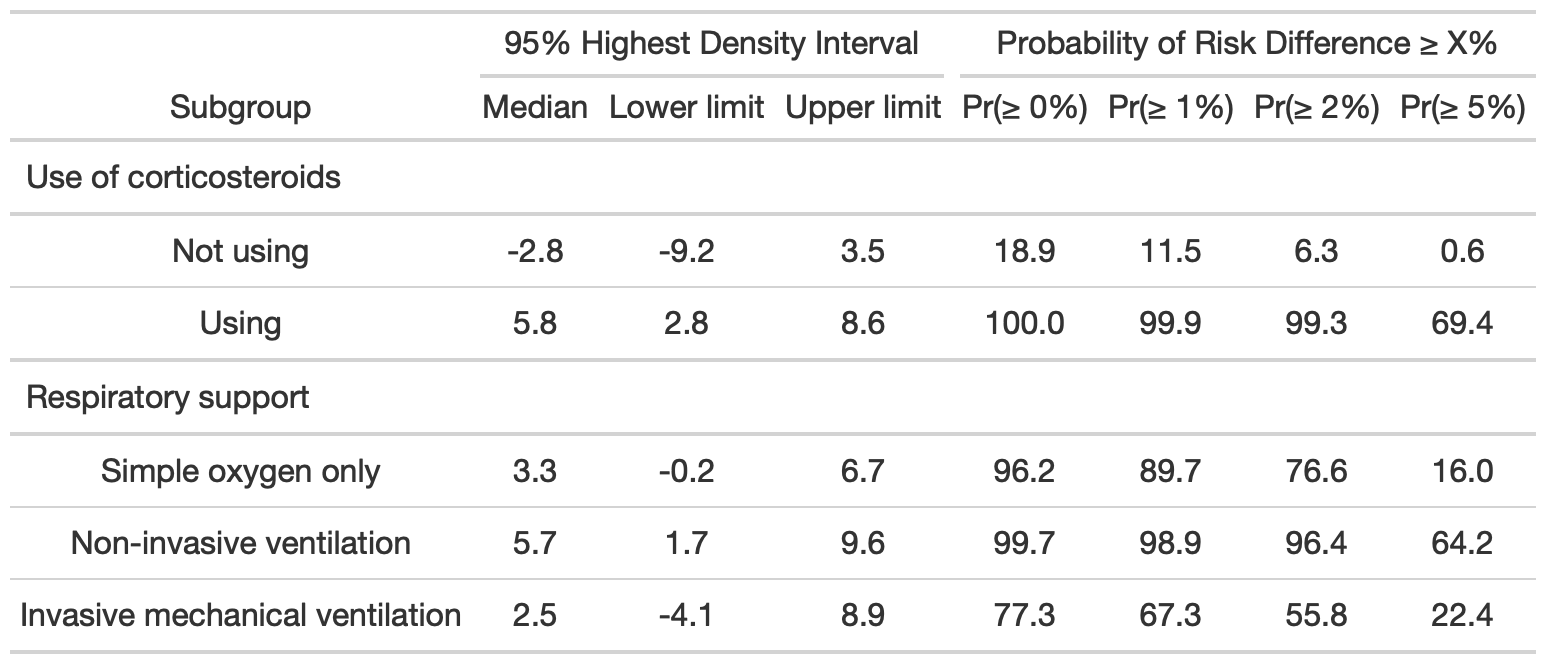
\includegraphics[width=0.9\linewidth]{/Users/arthur/Coding/projects/tocilizumab_reanalysis/final_analyses/output/plots/appendix/STable2_hdi_probabilities_figure2} \end{center}

95\% highest density intervals and posterior probabilities of benefit.
This table complements Figure 2.

\newpage

\hypertarget{sensitivity-analyses-using-different-priors}{%
\subsection{Sensitivity analyses using different
priors}\label{sensitivity-analyses-using-different-priors}}

\hypertarget{supplementary-figure-1}{%
\subsubsection{Supplementary Figure 1}\label{supplementary-figure-1}}

\begin{center}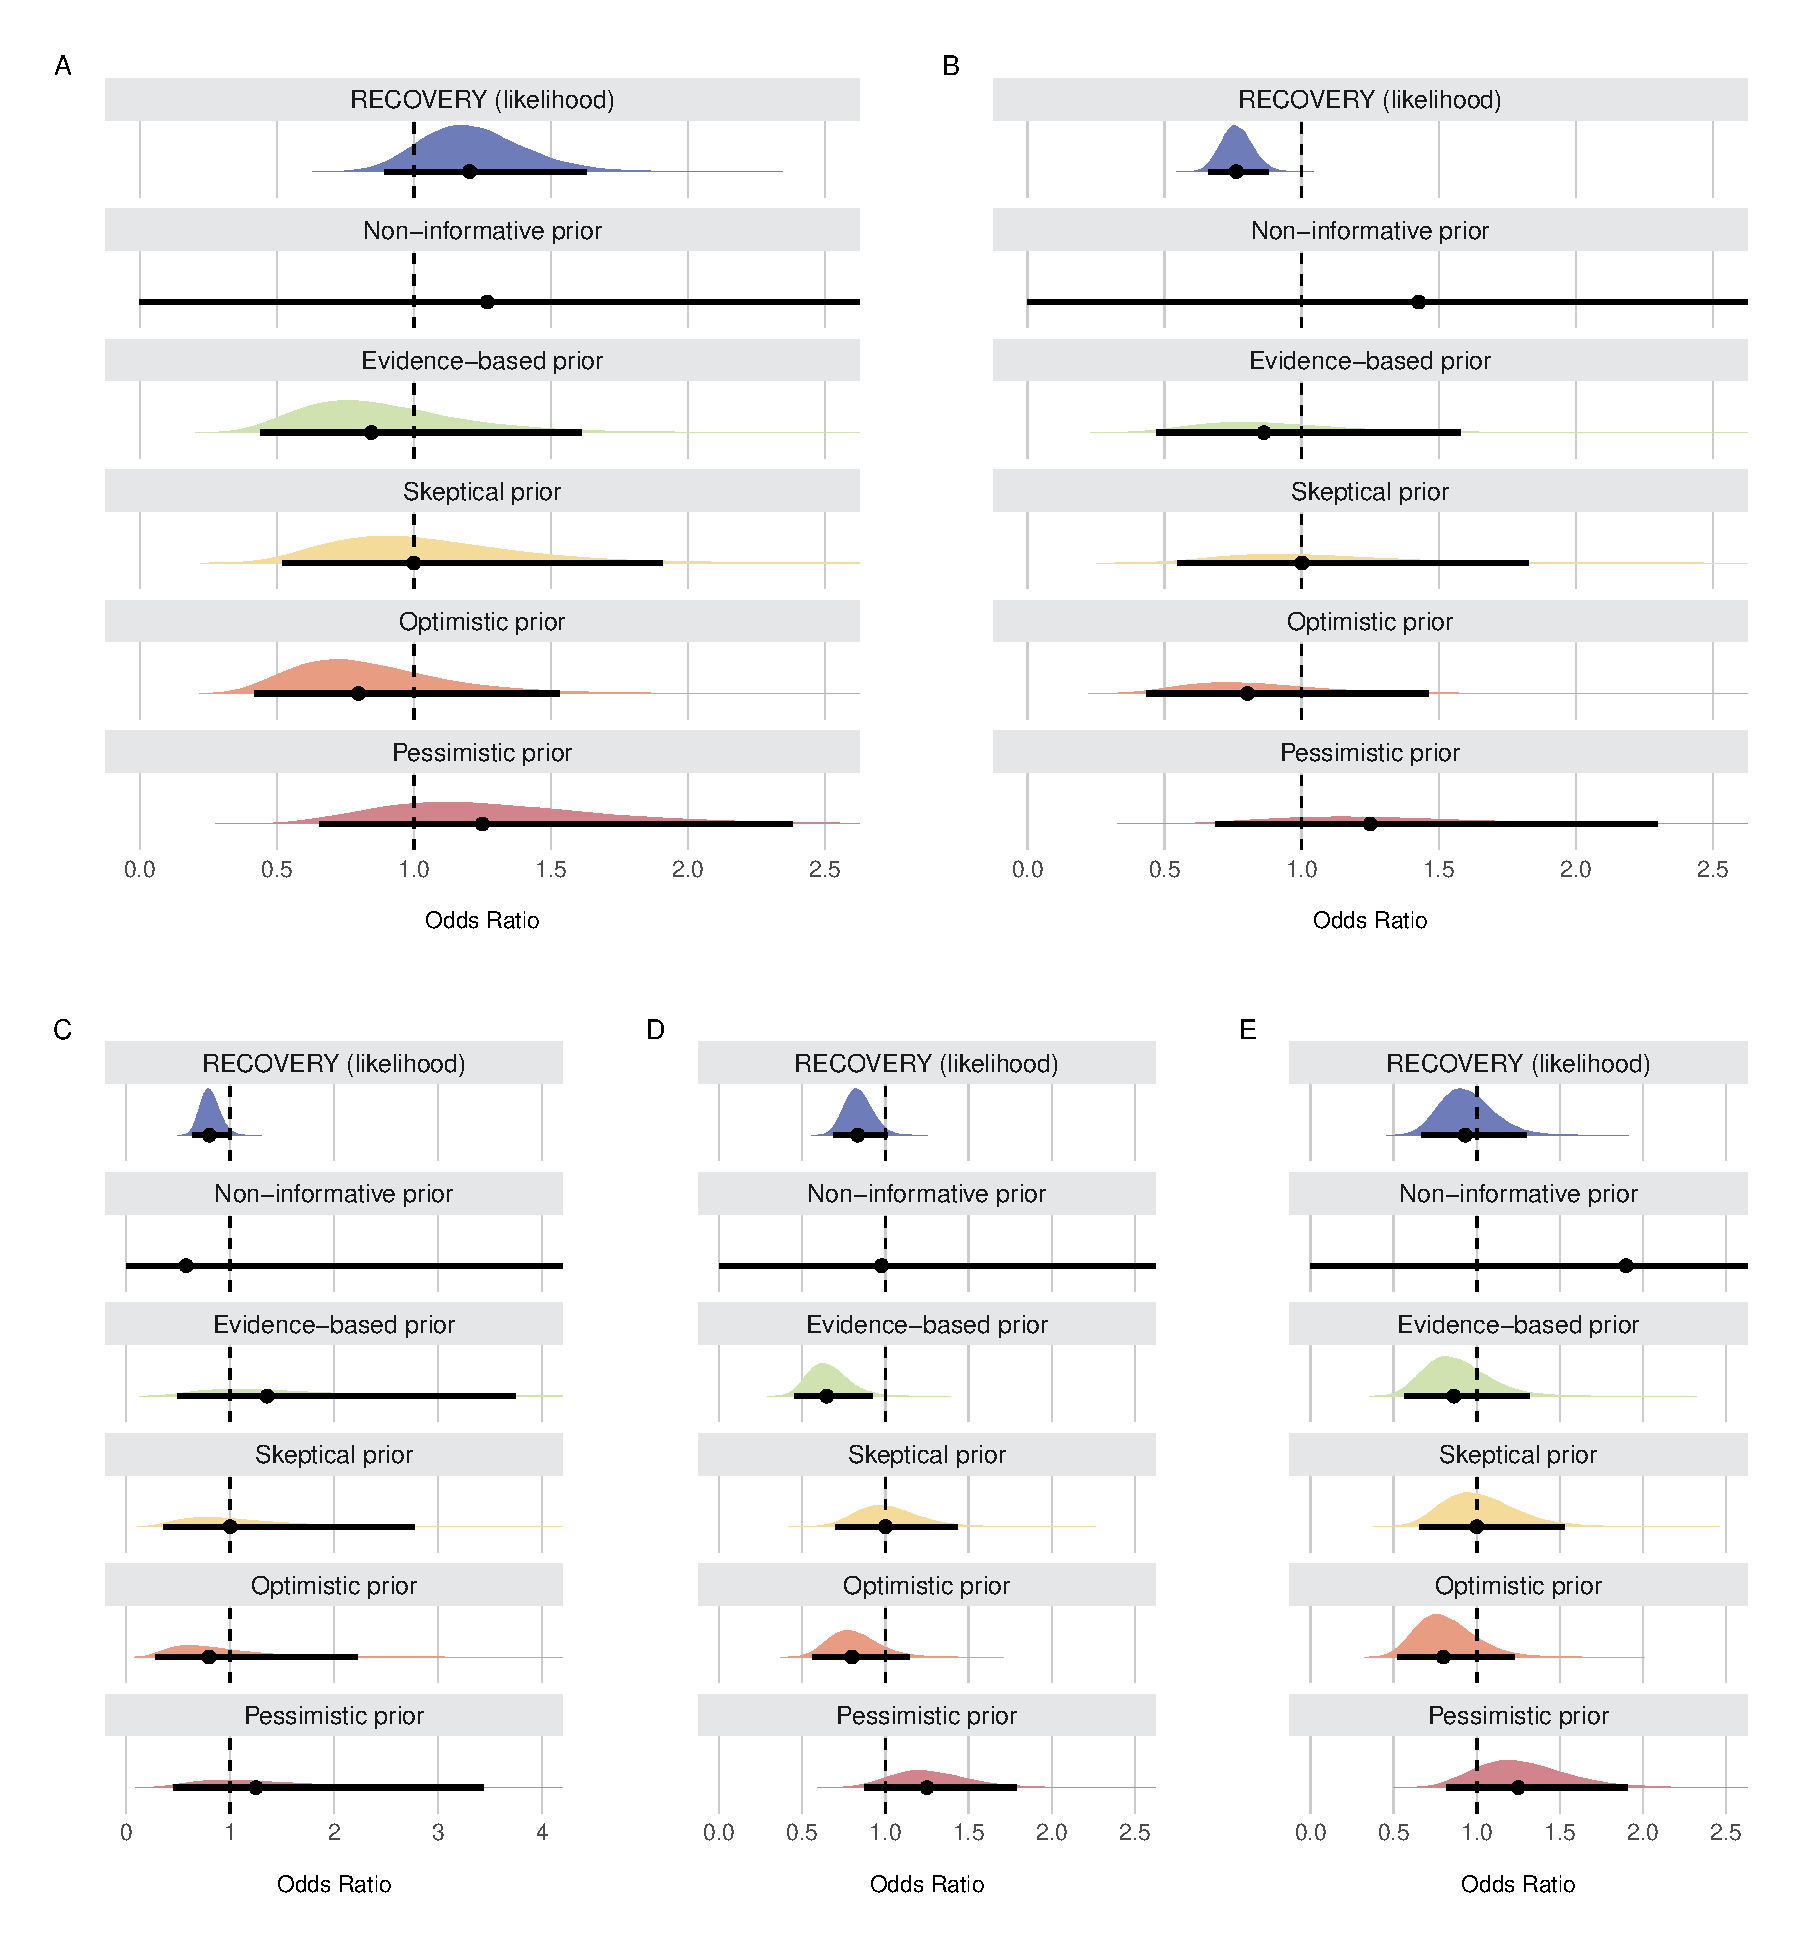
\includegraphics[width=0.95\linewidth]{/Users/arthur/Coding/projects/tocilizumab_reanalysis/final_analyses/output/plots/appendix/SFigure1_priors_sensitivity} \end{center}

Prior distributions for each subgroup.

Panel A shows results for patients not using corticosteroids; Panel B
shows results for patients using corticosteroids.

Panel C shows results for simple oxygen only; Panel D shows results for
non-invasive ventilation; Panel E shows results for invasive mechanical
ventilation.

Point estimates depict the median and interval bars depict 95th quantile
intervals.

\hypertarget{supplementary-table-3}{%
\subsubsection{Supplementary Table 3}\label{supplementary-table-3}}

\begin{center}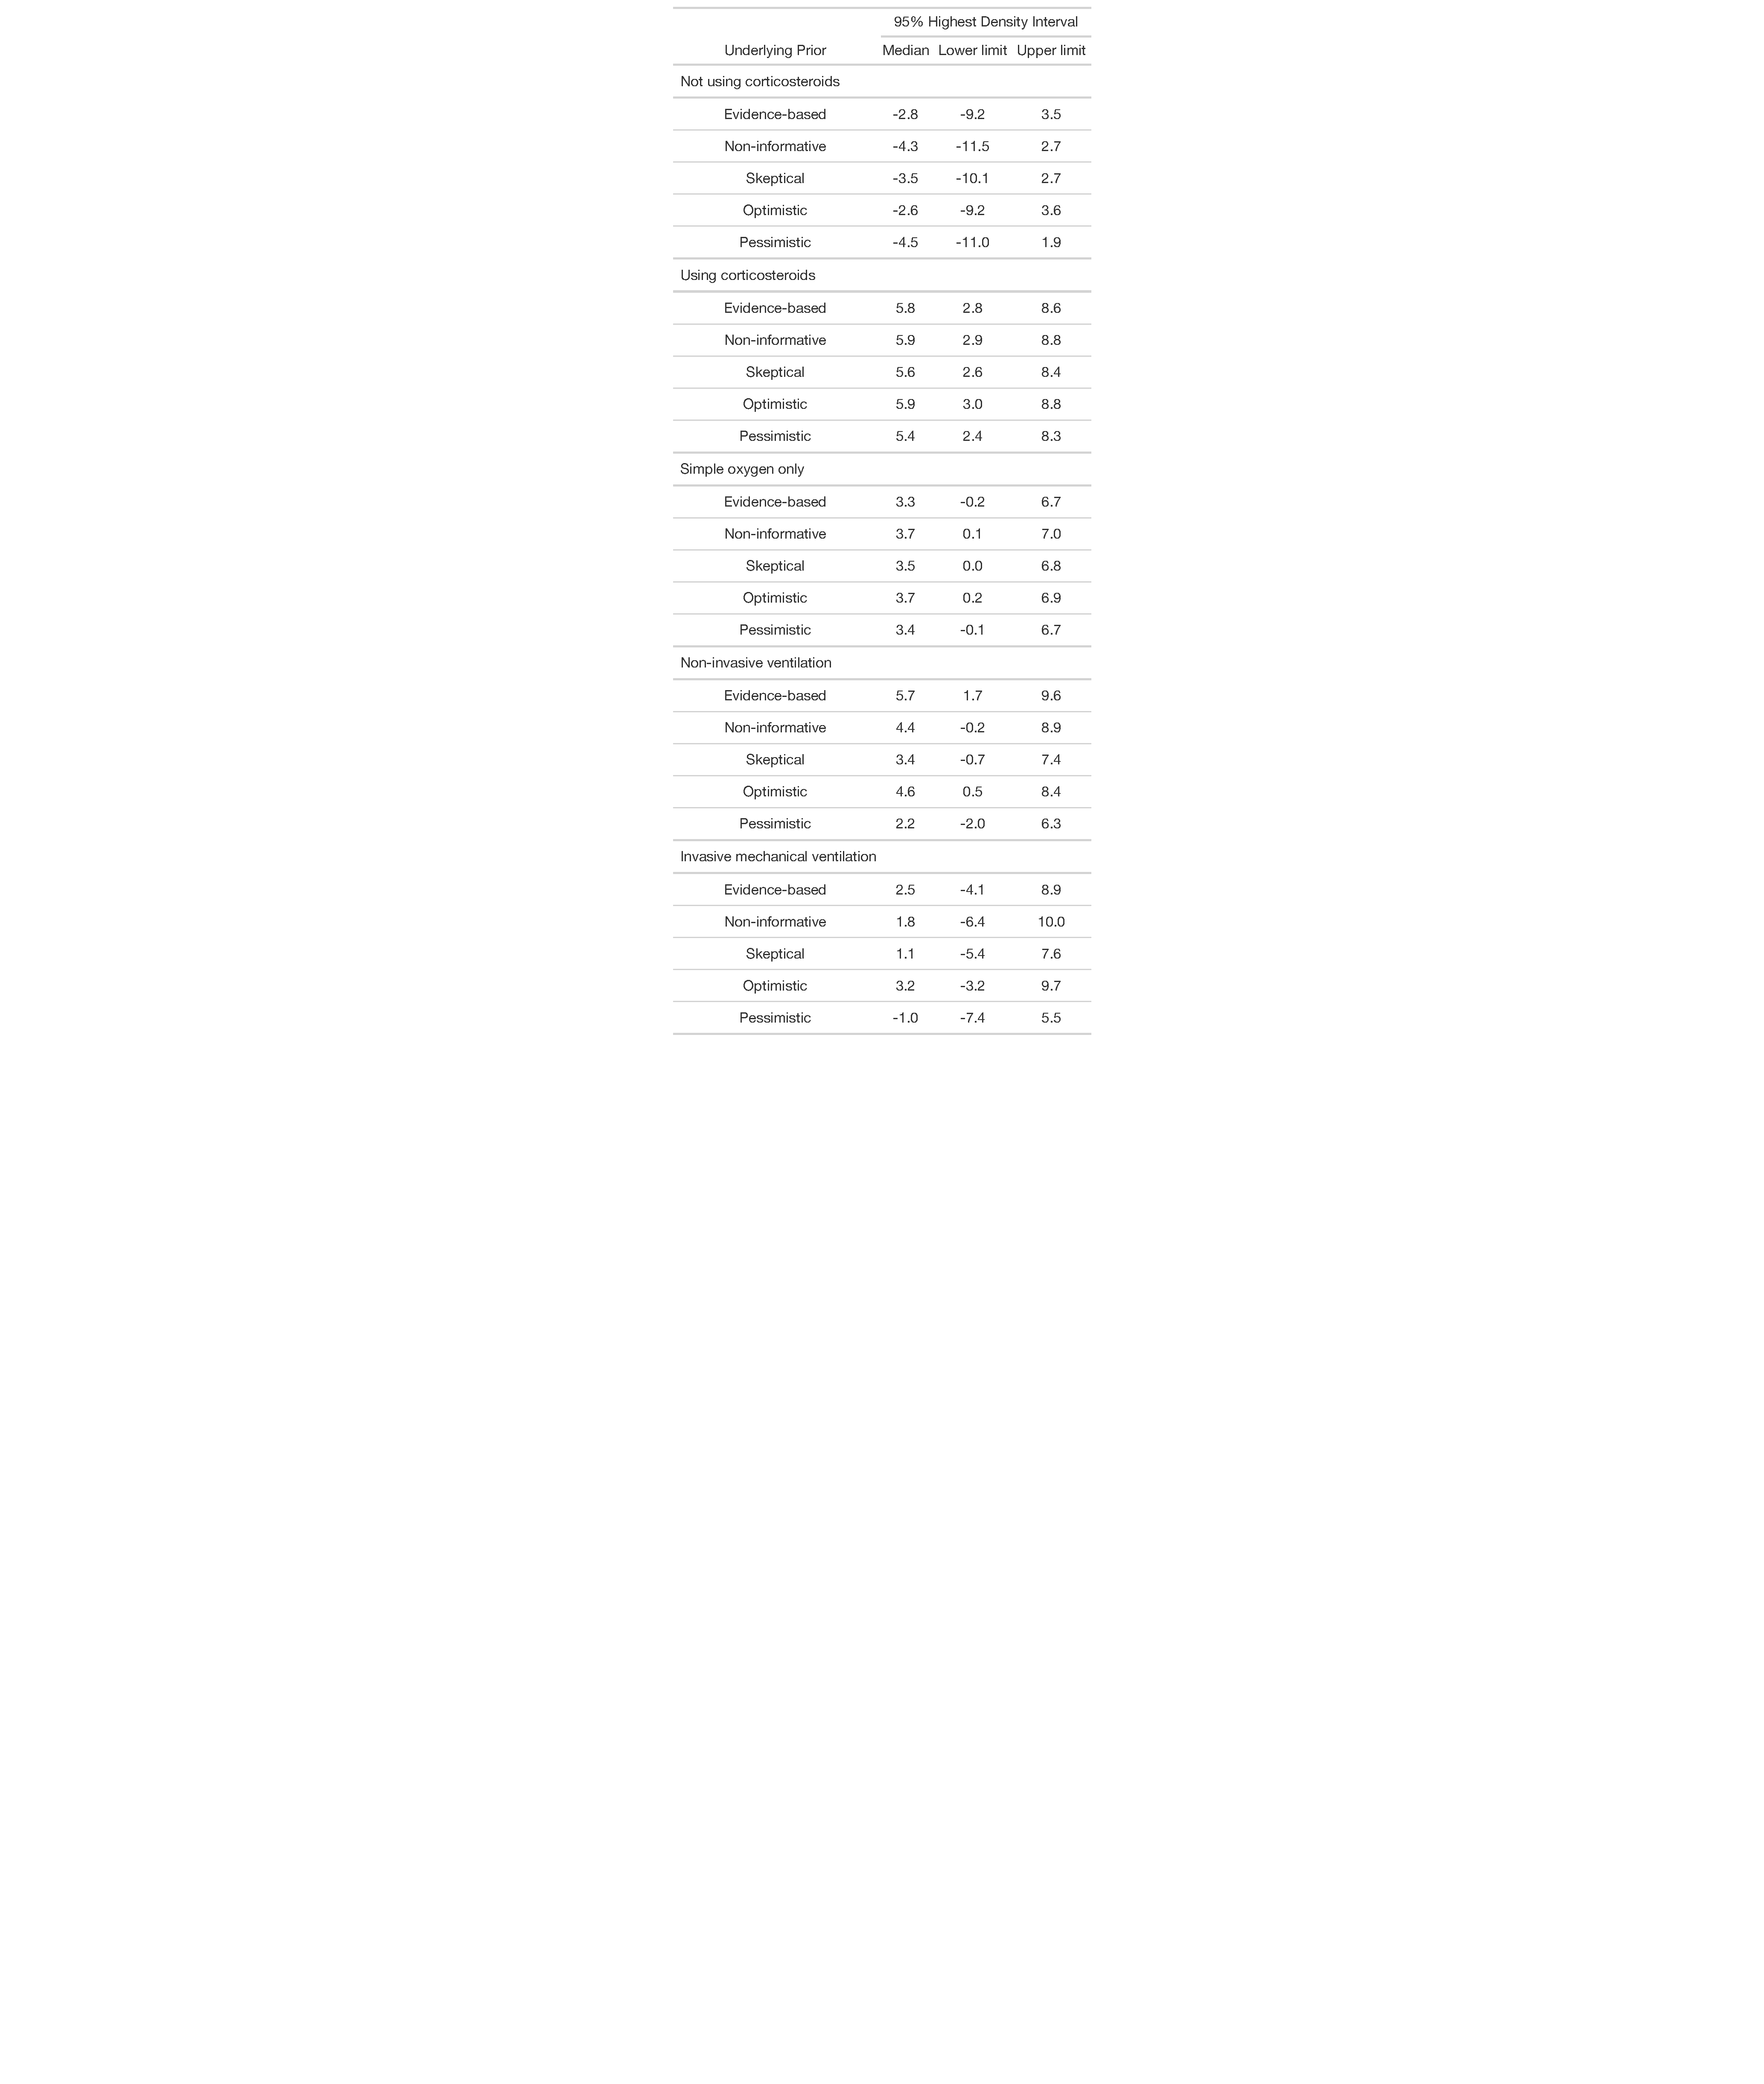
\includegraphics[width=0.5\linewidth]{/Users/arthur/Coding/projects/tocilizumab_reanalysis/final_analyses/output/plots/appendix/STable3_hdi_figure3} \end{center}

Median and 95\% highest density intervals of posteriors distributions
from sensitivity analyses with different priors. This table complements
Figure 3.

\hypertarget{supplementary-table-4}{%
\subsubsection{Supplementary Table 4}\label{supplementary-table-4}}

\begin{center}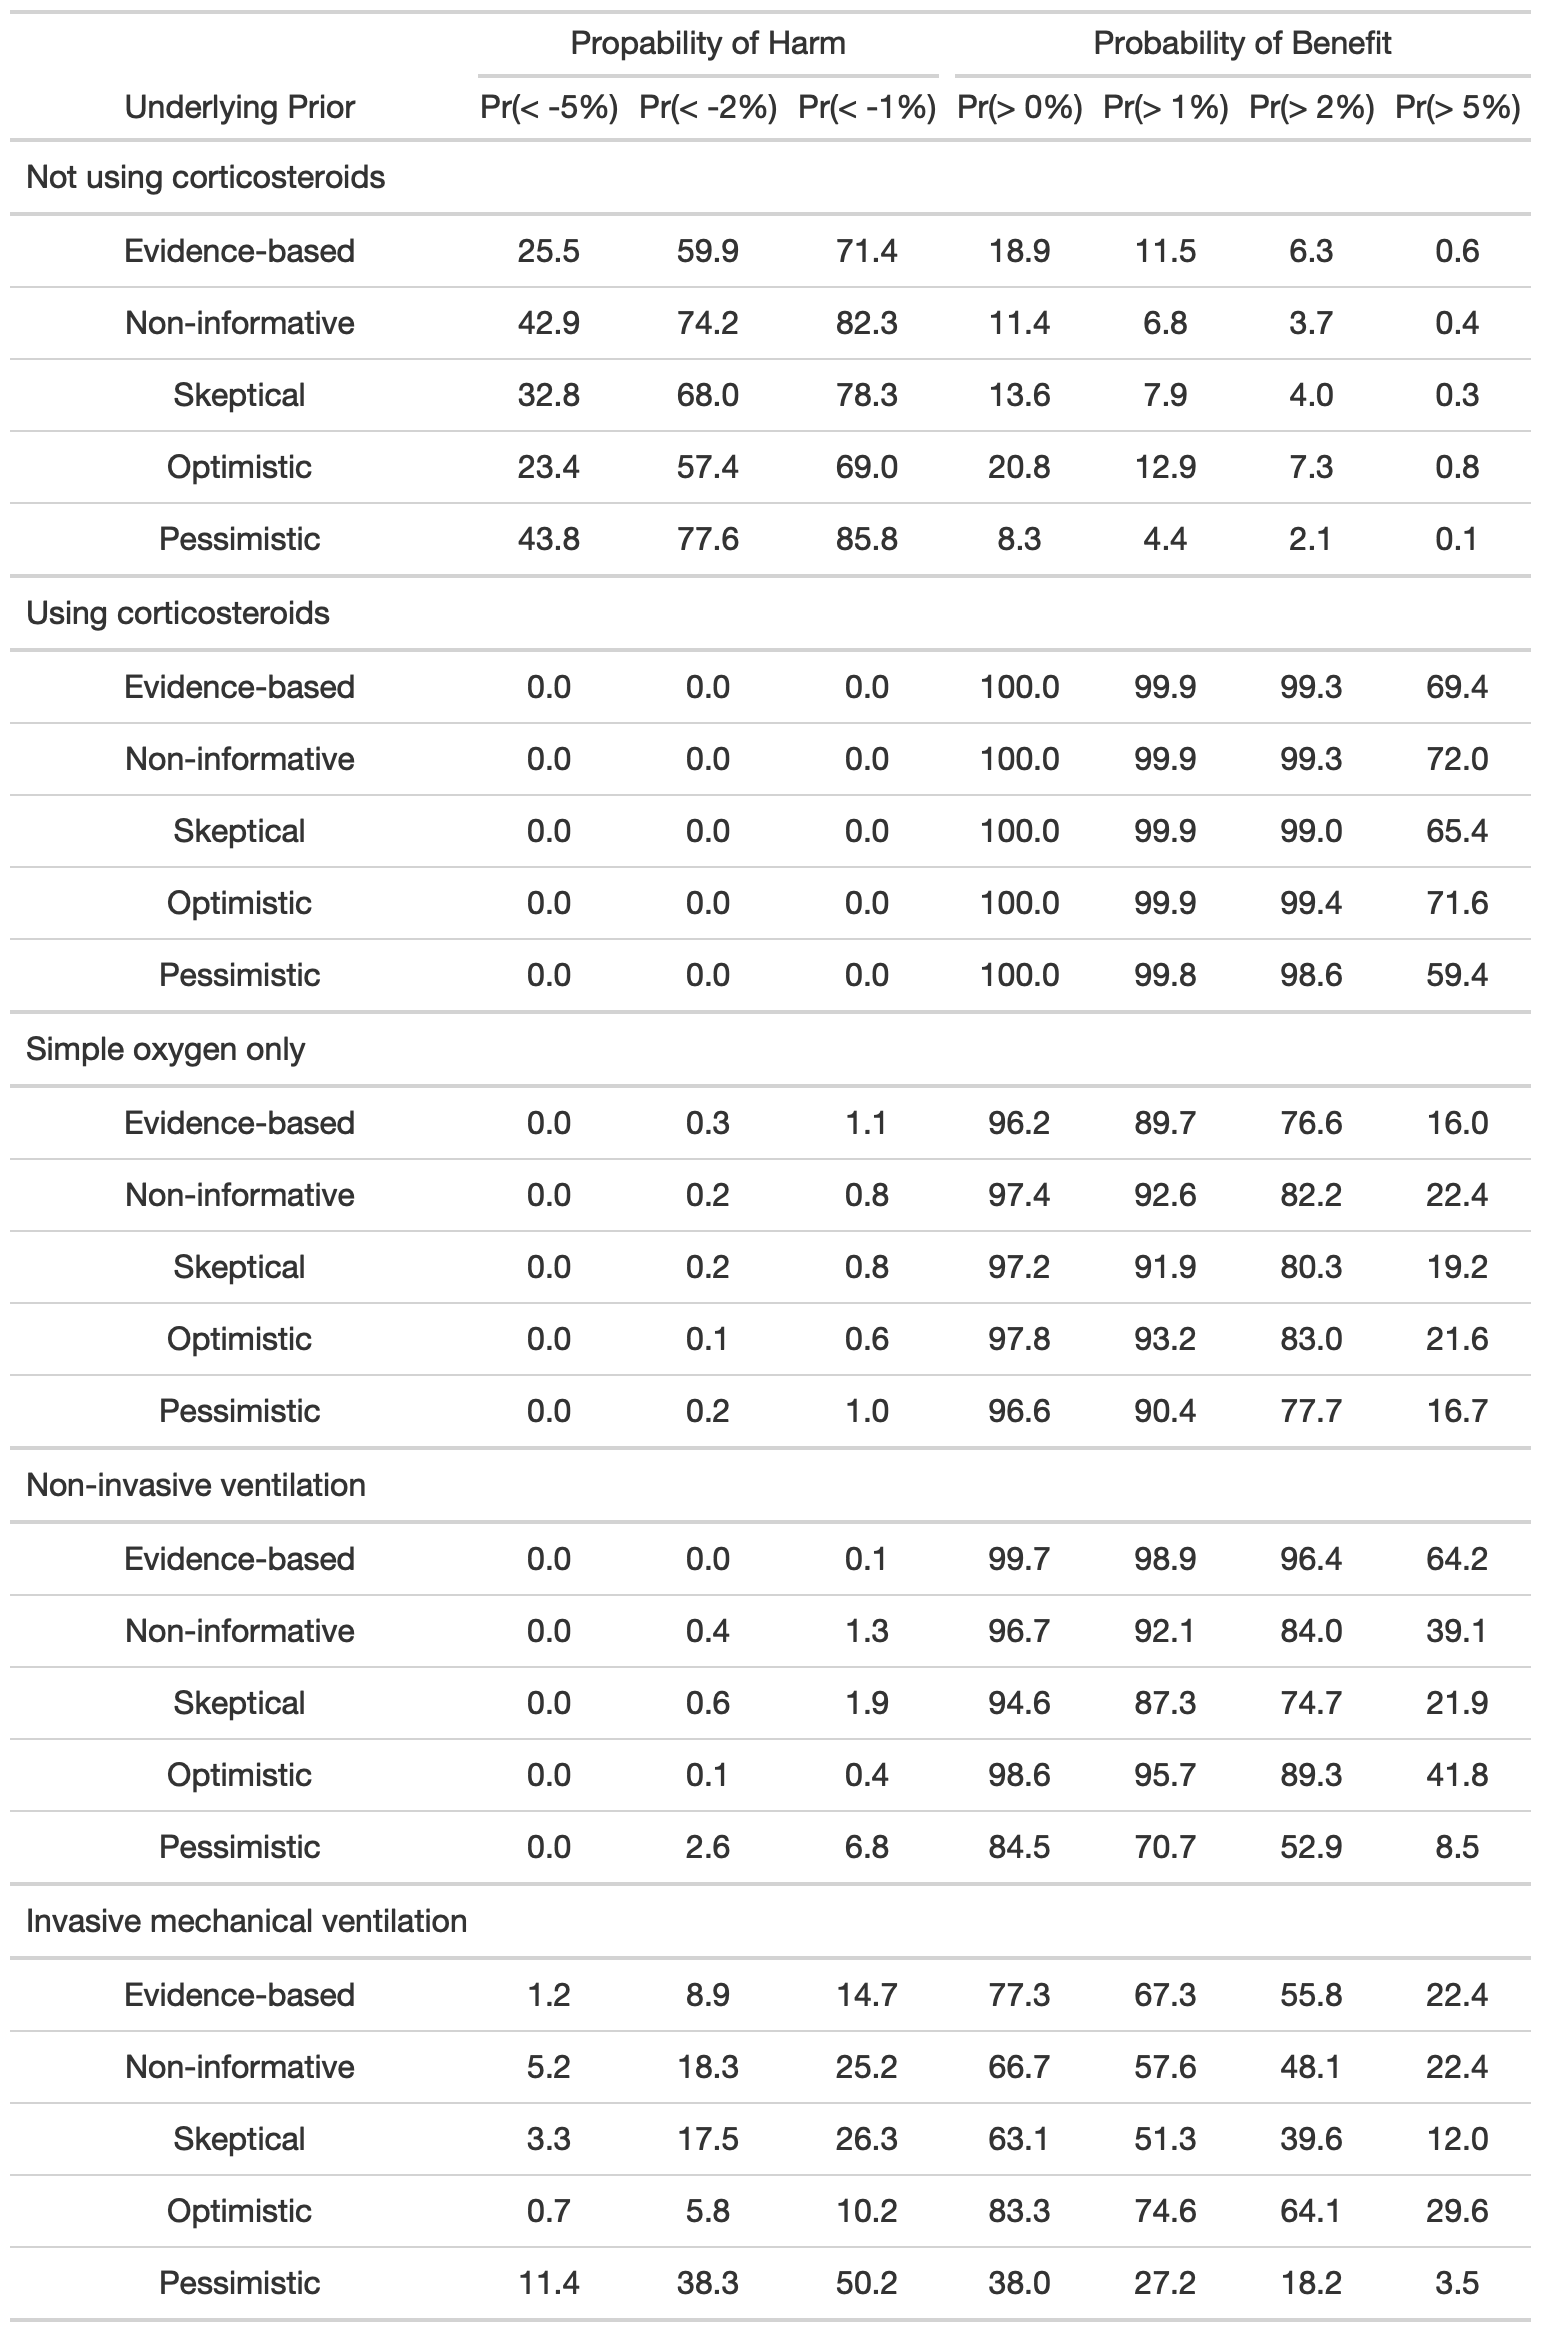
\includegraphics[width=0.8\linewidth]{/Users/arthur/Coding/projects/tocilizumab_reanalysis/final_analyses/output/plots/appendix/STable4_probabilities_figure3} \end{center}

Posterior probabilities from sensitivity analyses using different
priors. This table complements Figure 3.

\newpage

\hypertarget{sensitivity-analyses-using-different-baseline-risks}{%
\subsection{Sensitivity analyses using different baseline
risks}\label{sensitivity-analyses-using-different-baseline-risks}}

\hypertarget{supplementary-figure-2}{%
\subsubsection{Supplementary Figure 2}\label{supplementary-figure-2}}

\begin{center}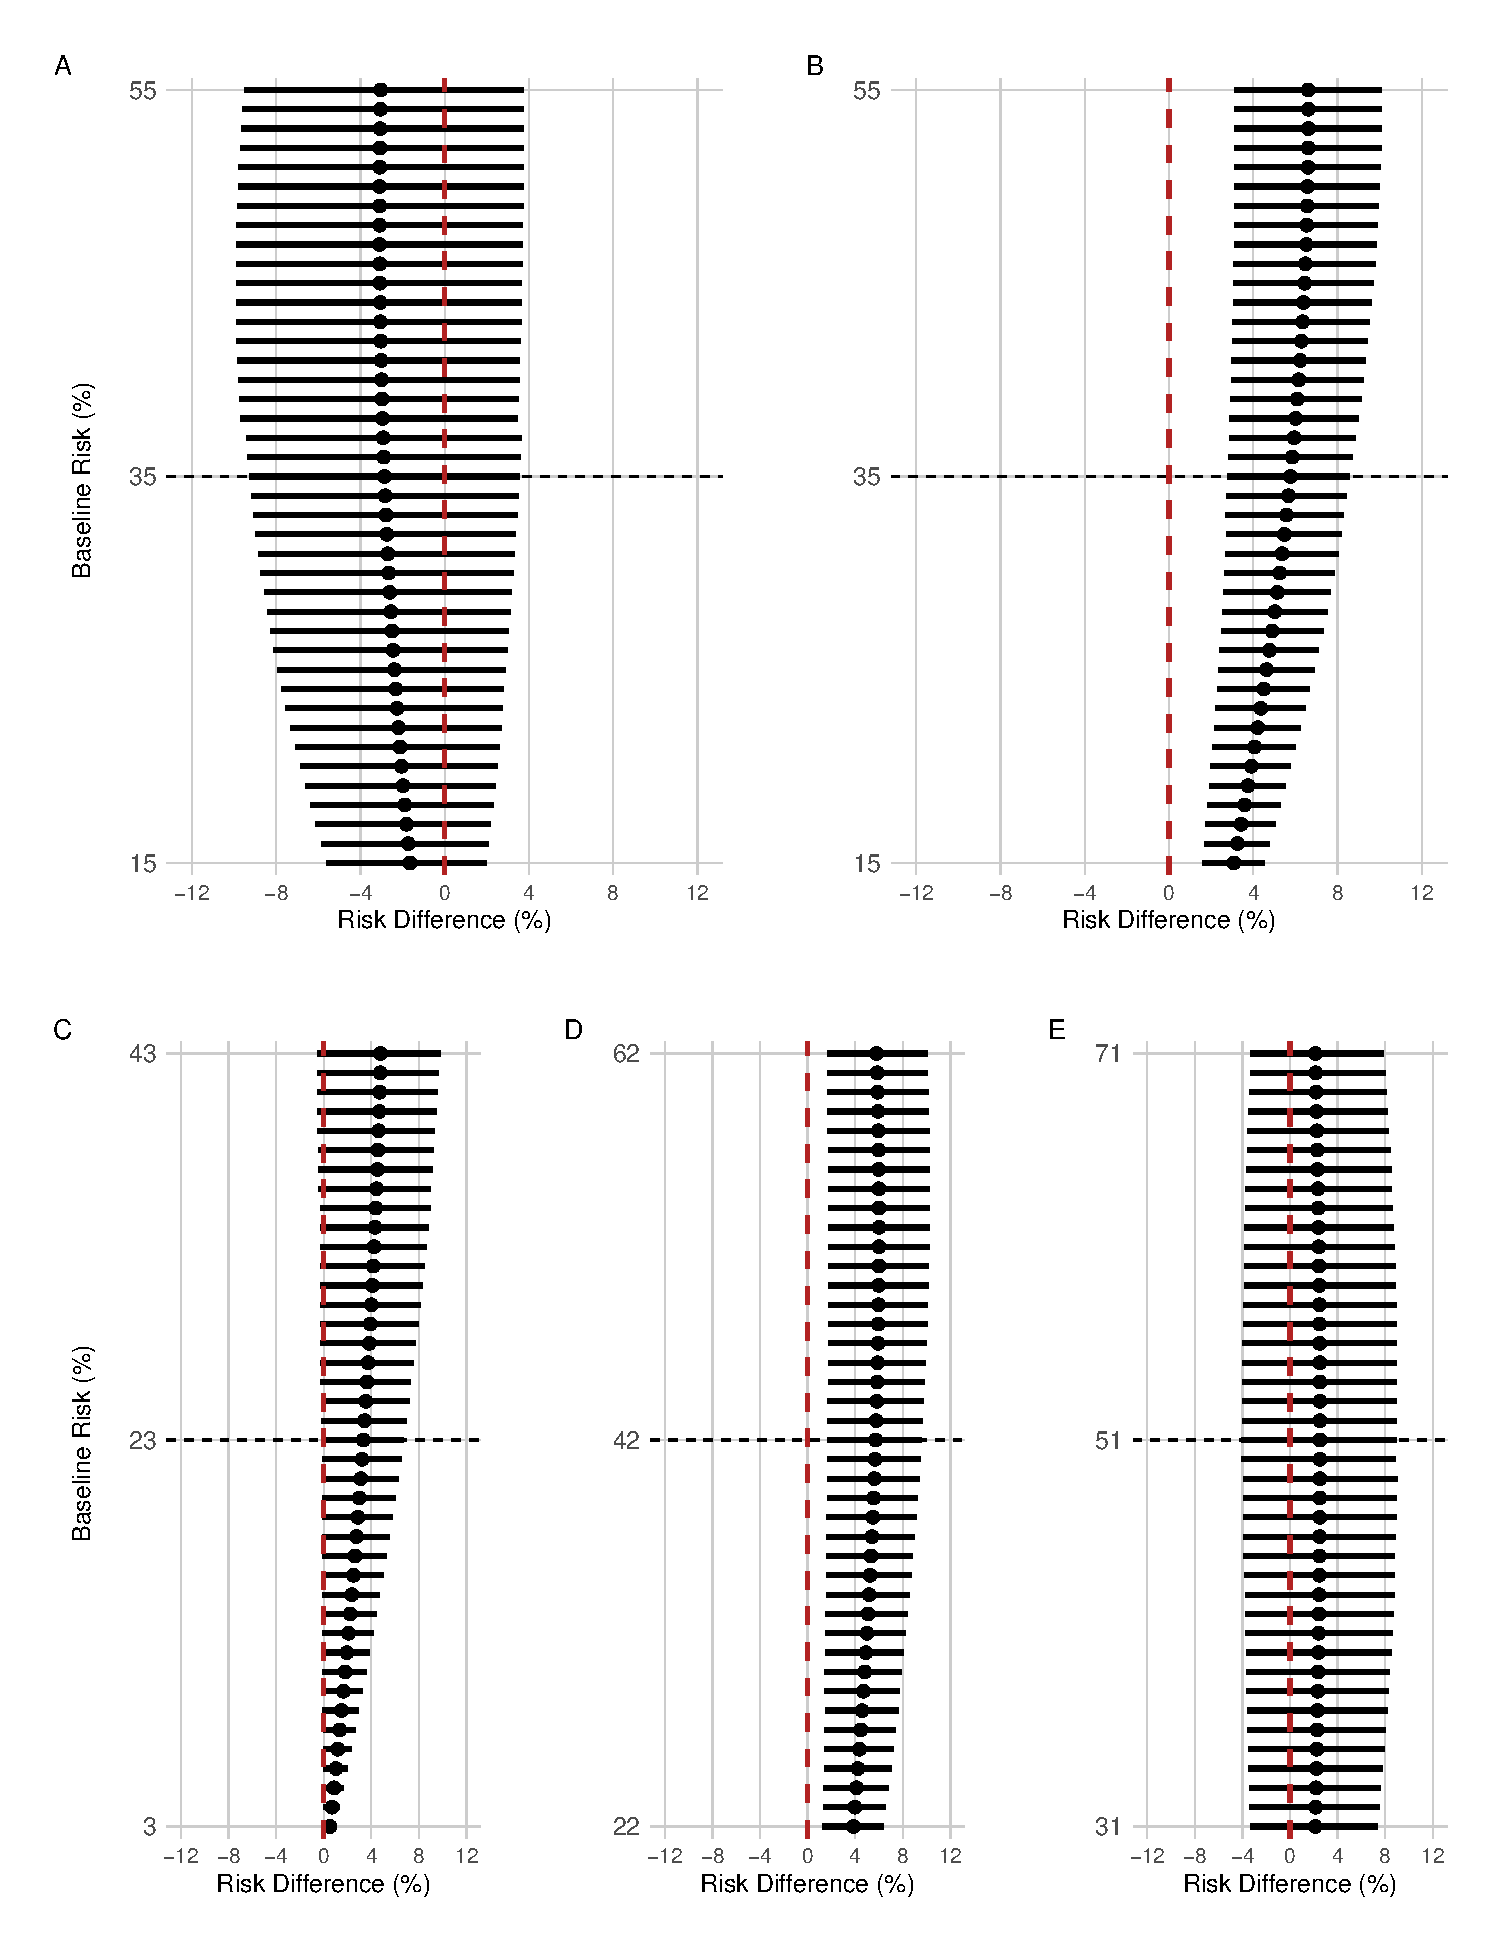
\includegraphics[width=0.7\linewidth]{/Users/arthur/Coding/projects/tocilizumab_reanalysis/final_analyses/output/plots/appendix/SFigure2_varying_baseline_risk_difference} \end{center}

Posterior distributions from sensitivity analyses using multiple
different baseline risks.

Each line represents posterior distribution for the corresponding
baseline risk. Horizontal black dashed lines represent the respective
baseline risk underlying other analyses (Figure 2), i.e., risk in the
control group in the RECOVERY trial for each subgroup (Table 1).
Vertical red dashed line represent 0\% risk difference. Point estimates
depict the median and interval bars depict 95\% highest density
intervals.

Panel A shows results for patients not using corticosteroids; Panel B
shows results for patients using corticosteroids. Panel C shows results
for simple oxygen only; Panel D shows results for non-invasive
ventilation; Panel E shows results for invasive mechanical ventilation.

\newpage

\hypertarget{results-hospital-discharge-outcome}{%
\section{Results: Hospital discharge
outcome}\label{results-hospital-discharge-outcome}}

\hypertarget{recovery-and-priors-number-of-events-and-sample-size}{%
\subsection{RECOVERY and Priors: Number of events and sample
size}\label{recovery-and-priors-number-of-events-and-sample-size}}

\hypertarget{supplementary-table-5}{%
\subsubsection{Supplementary Table 5}\label{supplementary-table-5}}

\begin{center}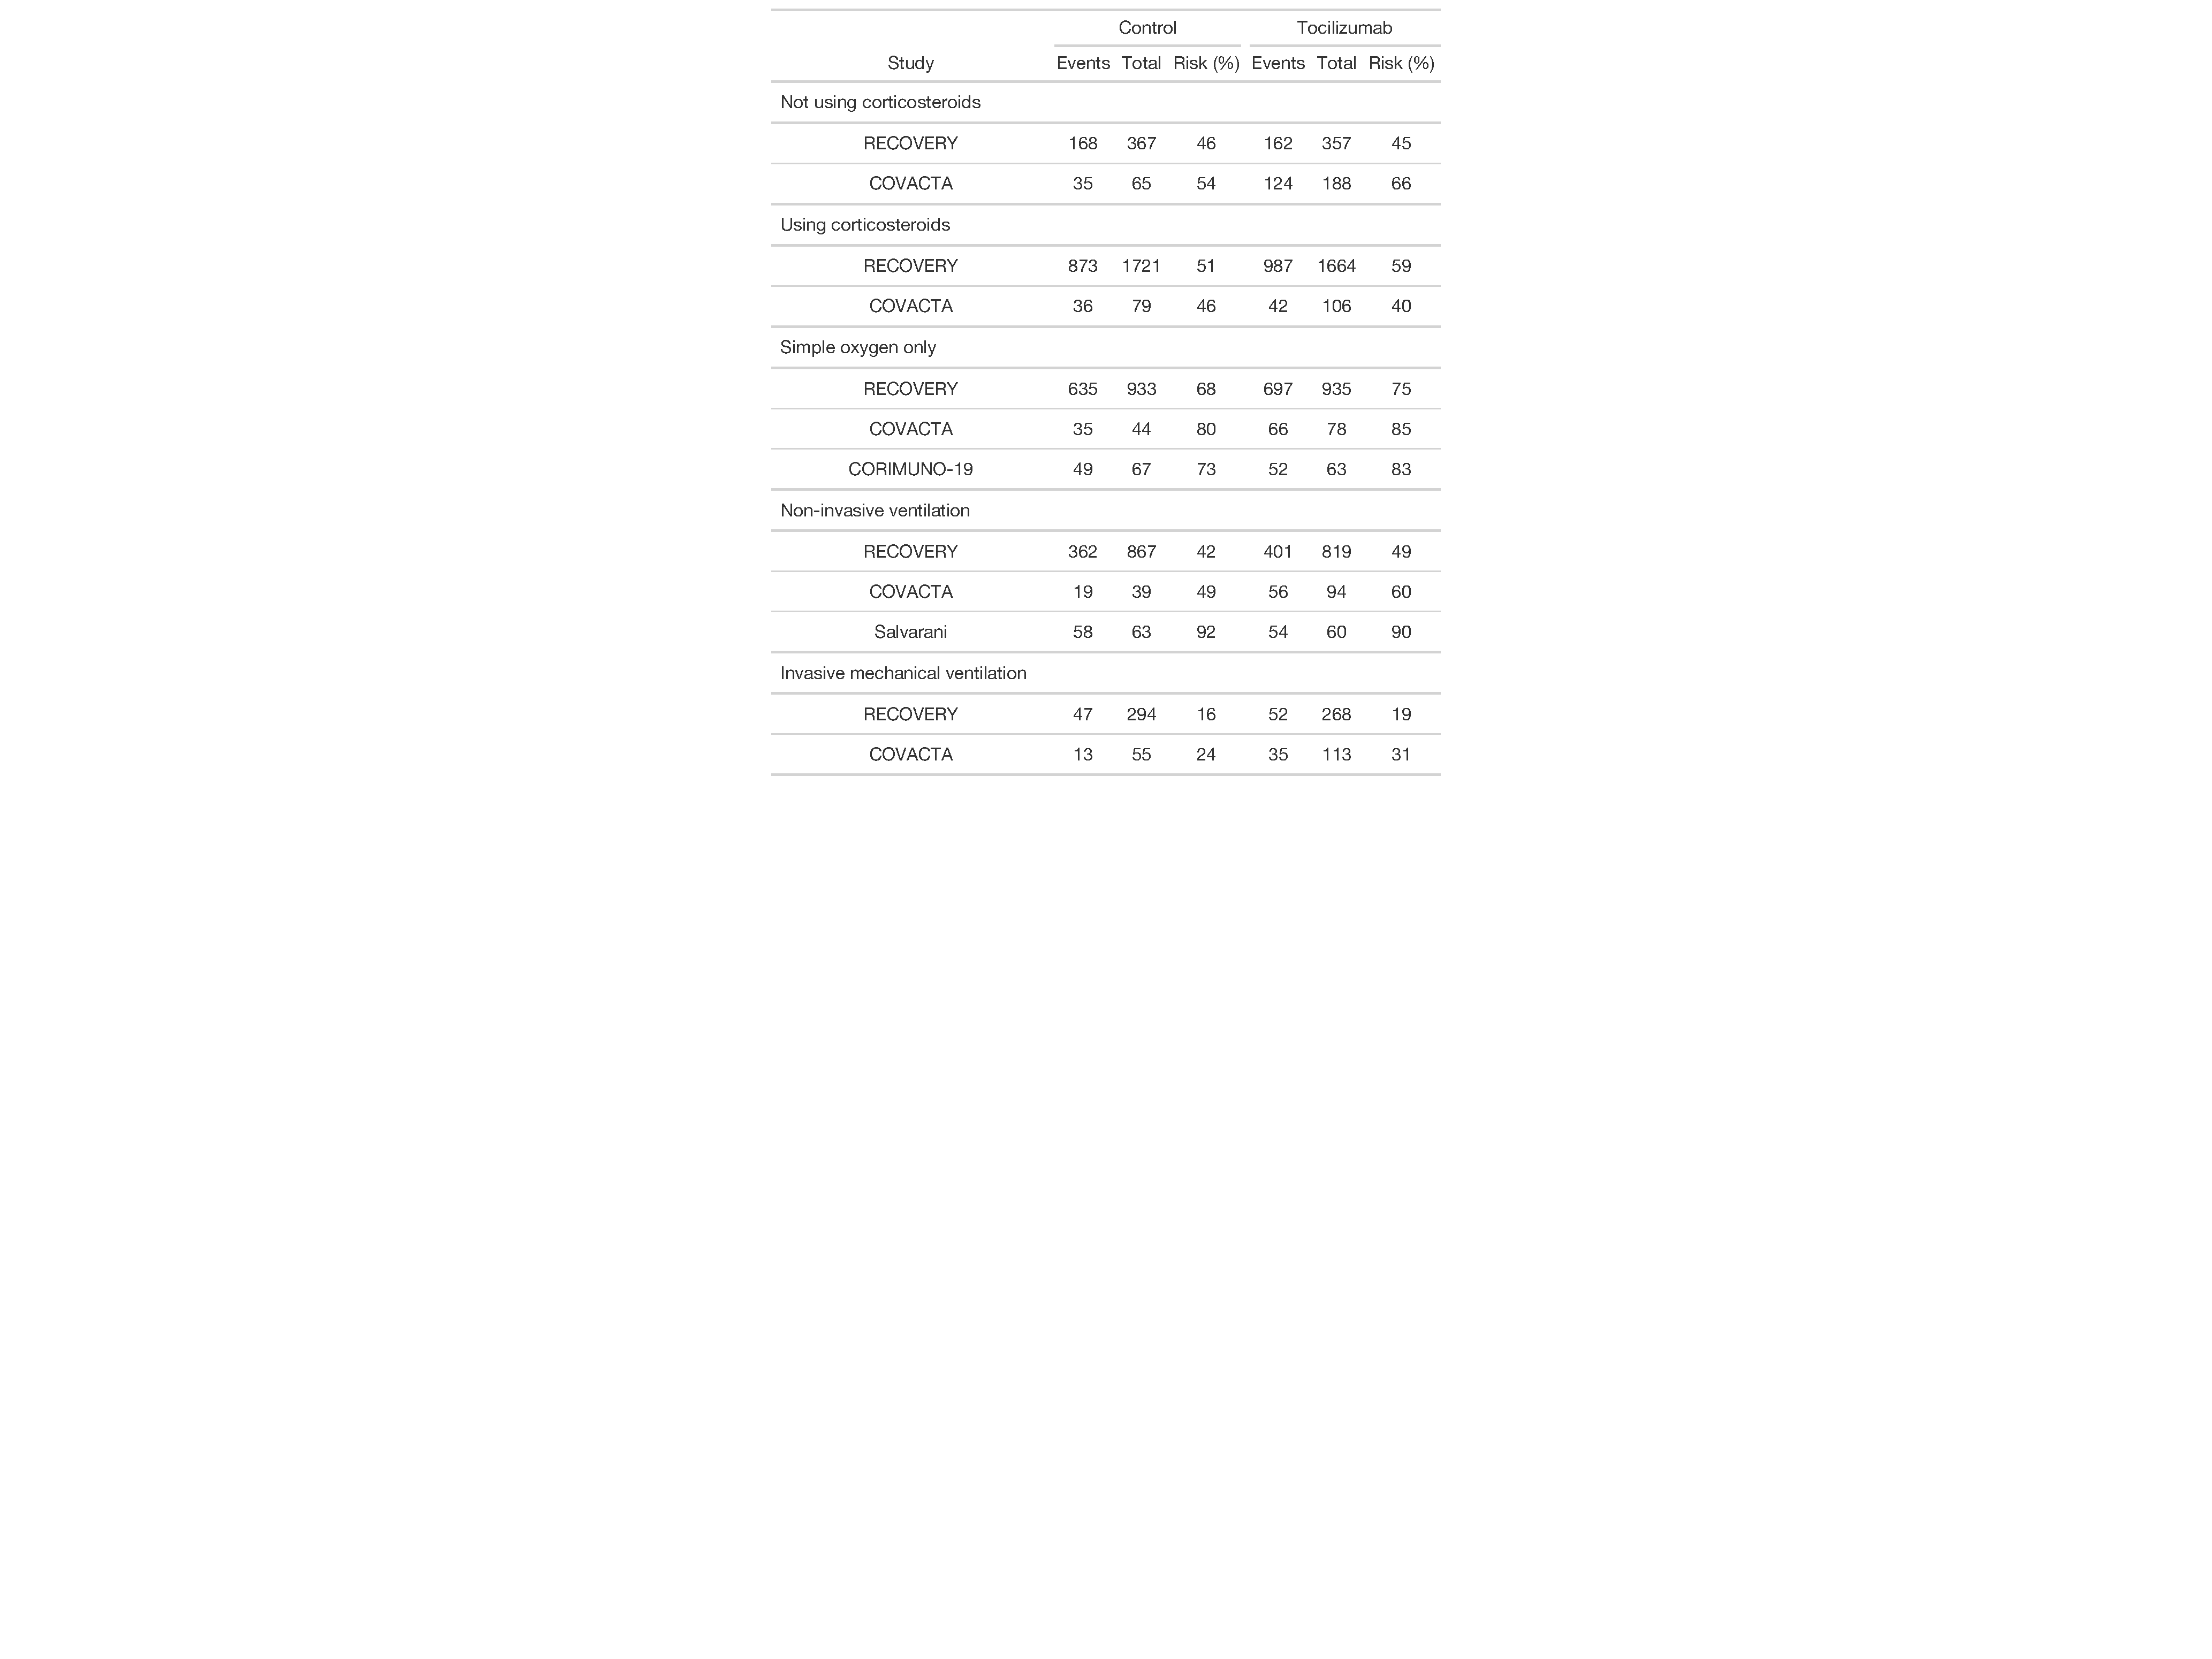
\includegraphics[width=0.9\linewidth]{/Users/arthur/Coding/projects/tocilizumab_reanalysis/final_analyses/output/plots/appendix/STable5_discharge_table1} \end{center}

\newpage

\hypertarget{prior-recovery-and-posterior-distributions-1}{%
\subsection{Prior, RECOVERY, and Posterior
distributions}\label{prior-recovery-and-posterior-distributions-1}}

\hypertarget{supplementary-figure-3}{%
\subsubsection{Supplementary Figure 3}\label{supplementary-figure-3}}

\begin{center}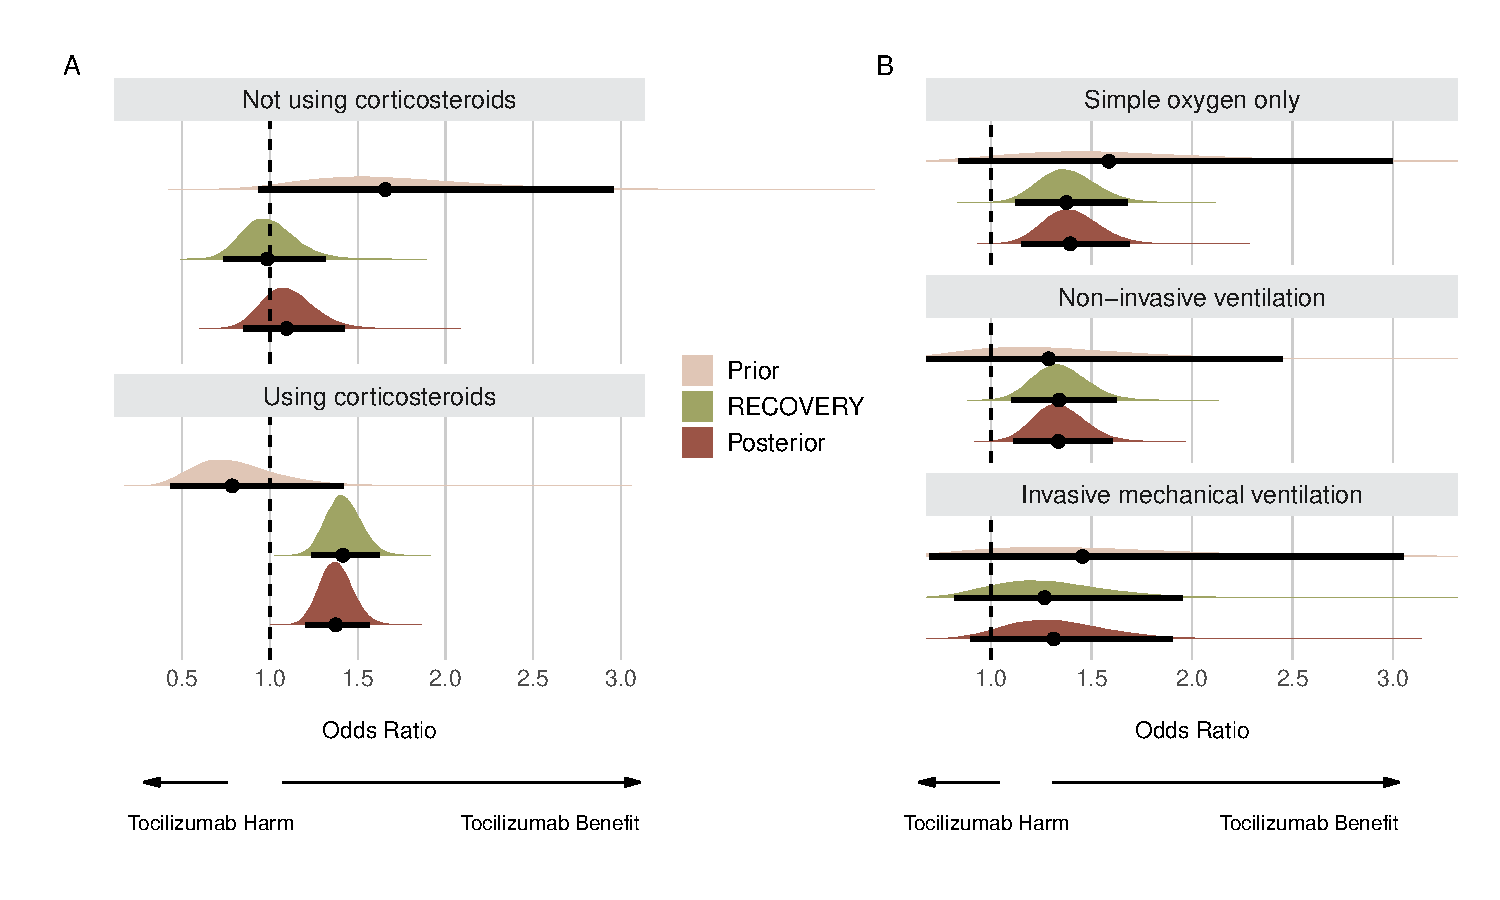
\includegraphics[width=1.1\linewidth]{/Users/arthur/Coding/projects/tocilizumab_reanalysis/final_analyses/output/plots/appendix/SFigure3_discharge_figure1} \end{center}

Point estimates depict the median and interval bars depict 95\% highest
density intervals.

\hypertarget{supplementary-table-6}{%
\subsubsection{Supplementary Table 6}\label{supplementary-table-6}}

\begin{center}\includegraphics[width=0.6\linewidth]{/Users/arthur/Coding/projects/tocilizumab_reanalysis/final_analyses/output/plots/appendix/STable6_discharge_HDI_intervals_figureS3} \end{center}

95\% highest density intervals of evidence-based prior, RECOVERY, and
posterior distributions. This table complements Supplementary Figure 3.

\newpage

\hypertarget{posterior-distribution-and-probabilities-using-evidence-based-priors}{%
\subsection{Posterior distribution and probabilities using
evidence-based
priors}\label{posterior-distribution-and-probabilities-using-evidence-based-priors}}

\hypertarget{supplementary-figure-4}{%
\subsubsection{Supplementary Figure 4}\label{supplementary-figure-4}}

\begin{center}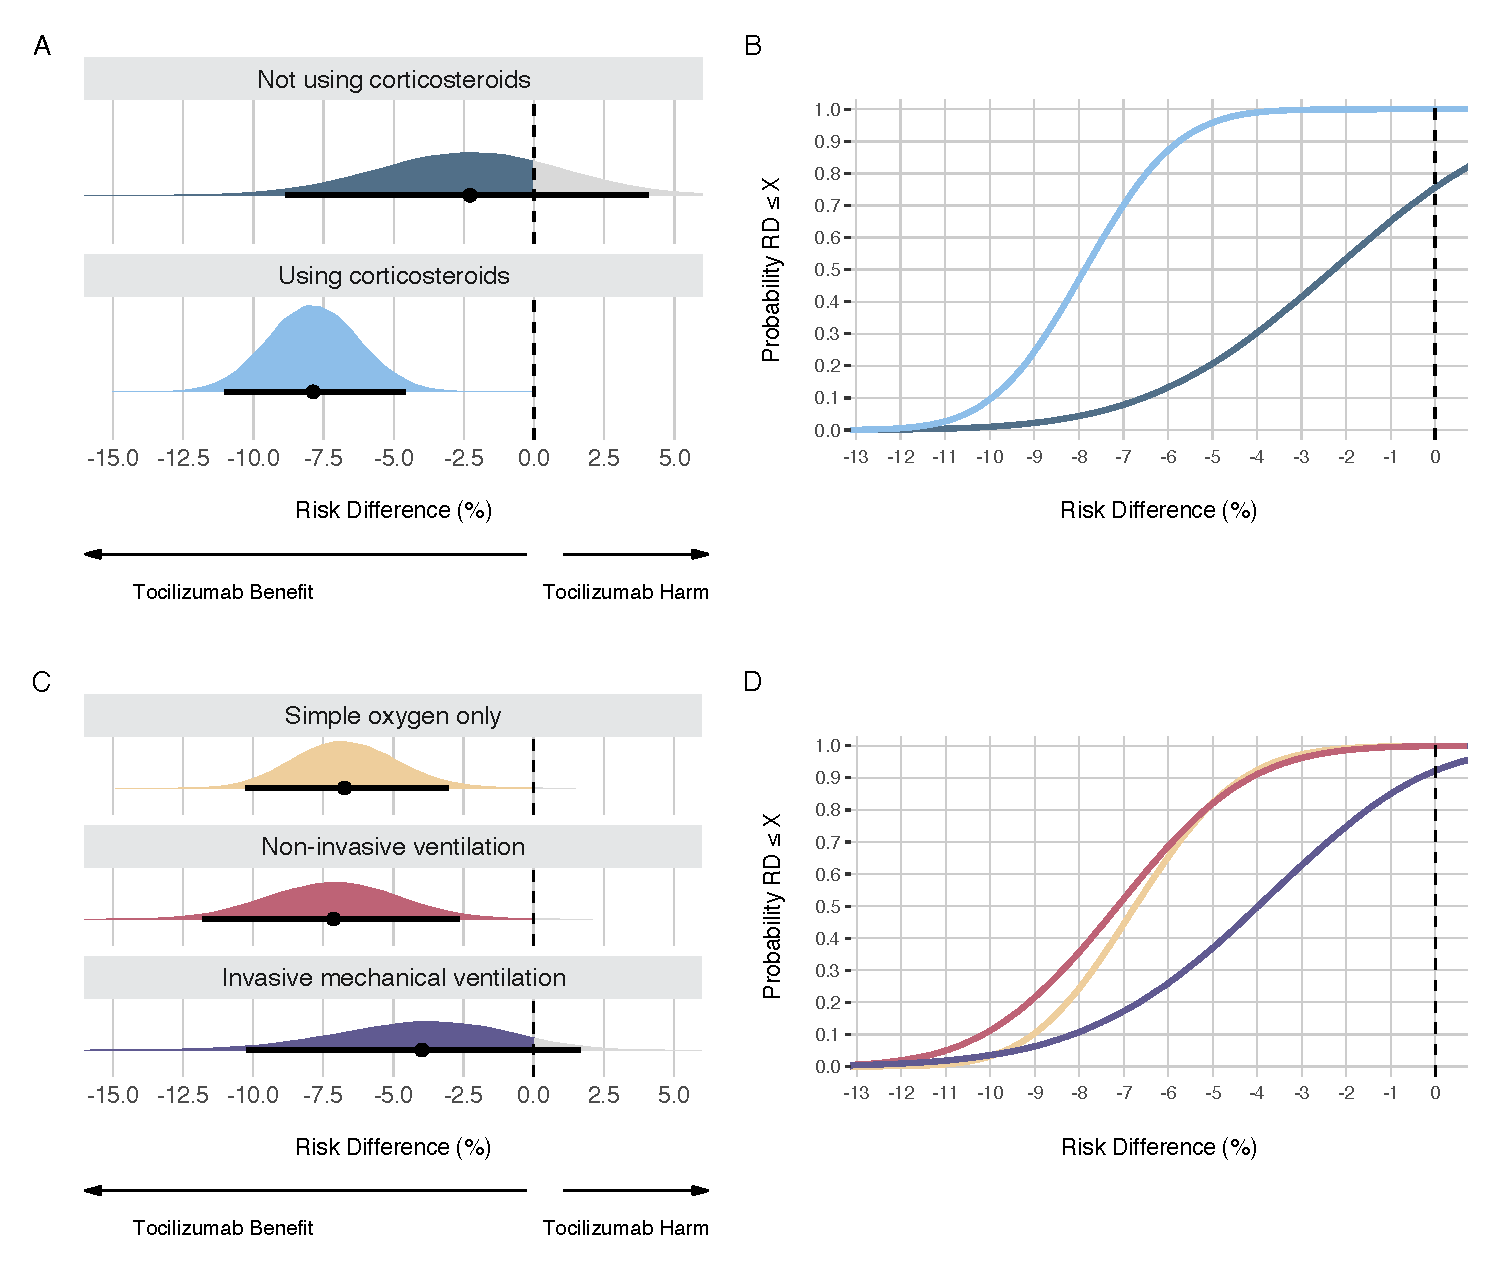
\includegraphics[width=1\linewidth]{/Users/arthur/Coding/projects/tocilizumab_reanalysis/final_analyses/output/plots/appendix/SFigure4_discharge_figure2} \end{center}

Panels A and C: Point estimates depict the median. Interval bars depict
the 80 and 95\% highest density intervals. Panels B and D: Cumulative
posterior distributions correspond to the probabilities that the risk
difference (RD) is lower than or equal to the effect size on the X‐axis.
The colors in Panels B and D match the ones used in Panels A and C.

\newpage

\hypertarget{sensitivity-analyses-using-different-priors-1}{%
\subsection{Sensitivity analyses using different
priors}\label{sensitivity-analyses-using-different-priors-1}}

\hypertarget{supplementary-figure-5}{%
\subsubsection{Supplementary Figure 5}\label{supplementary-figure-5}}

\begin{center}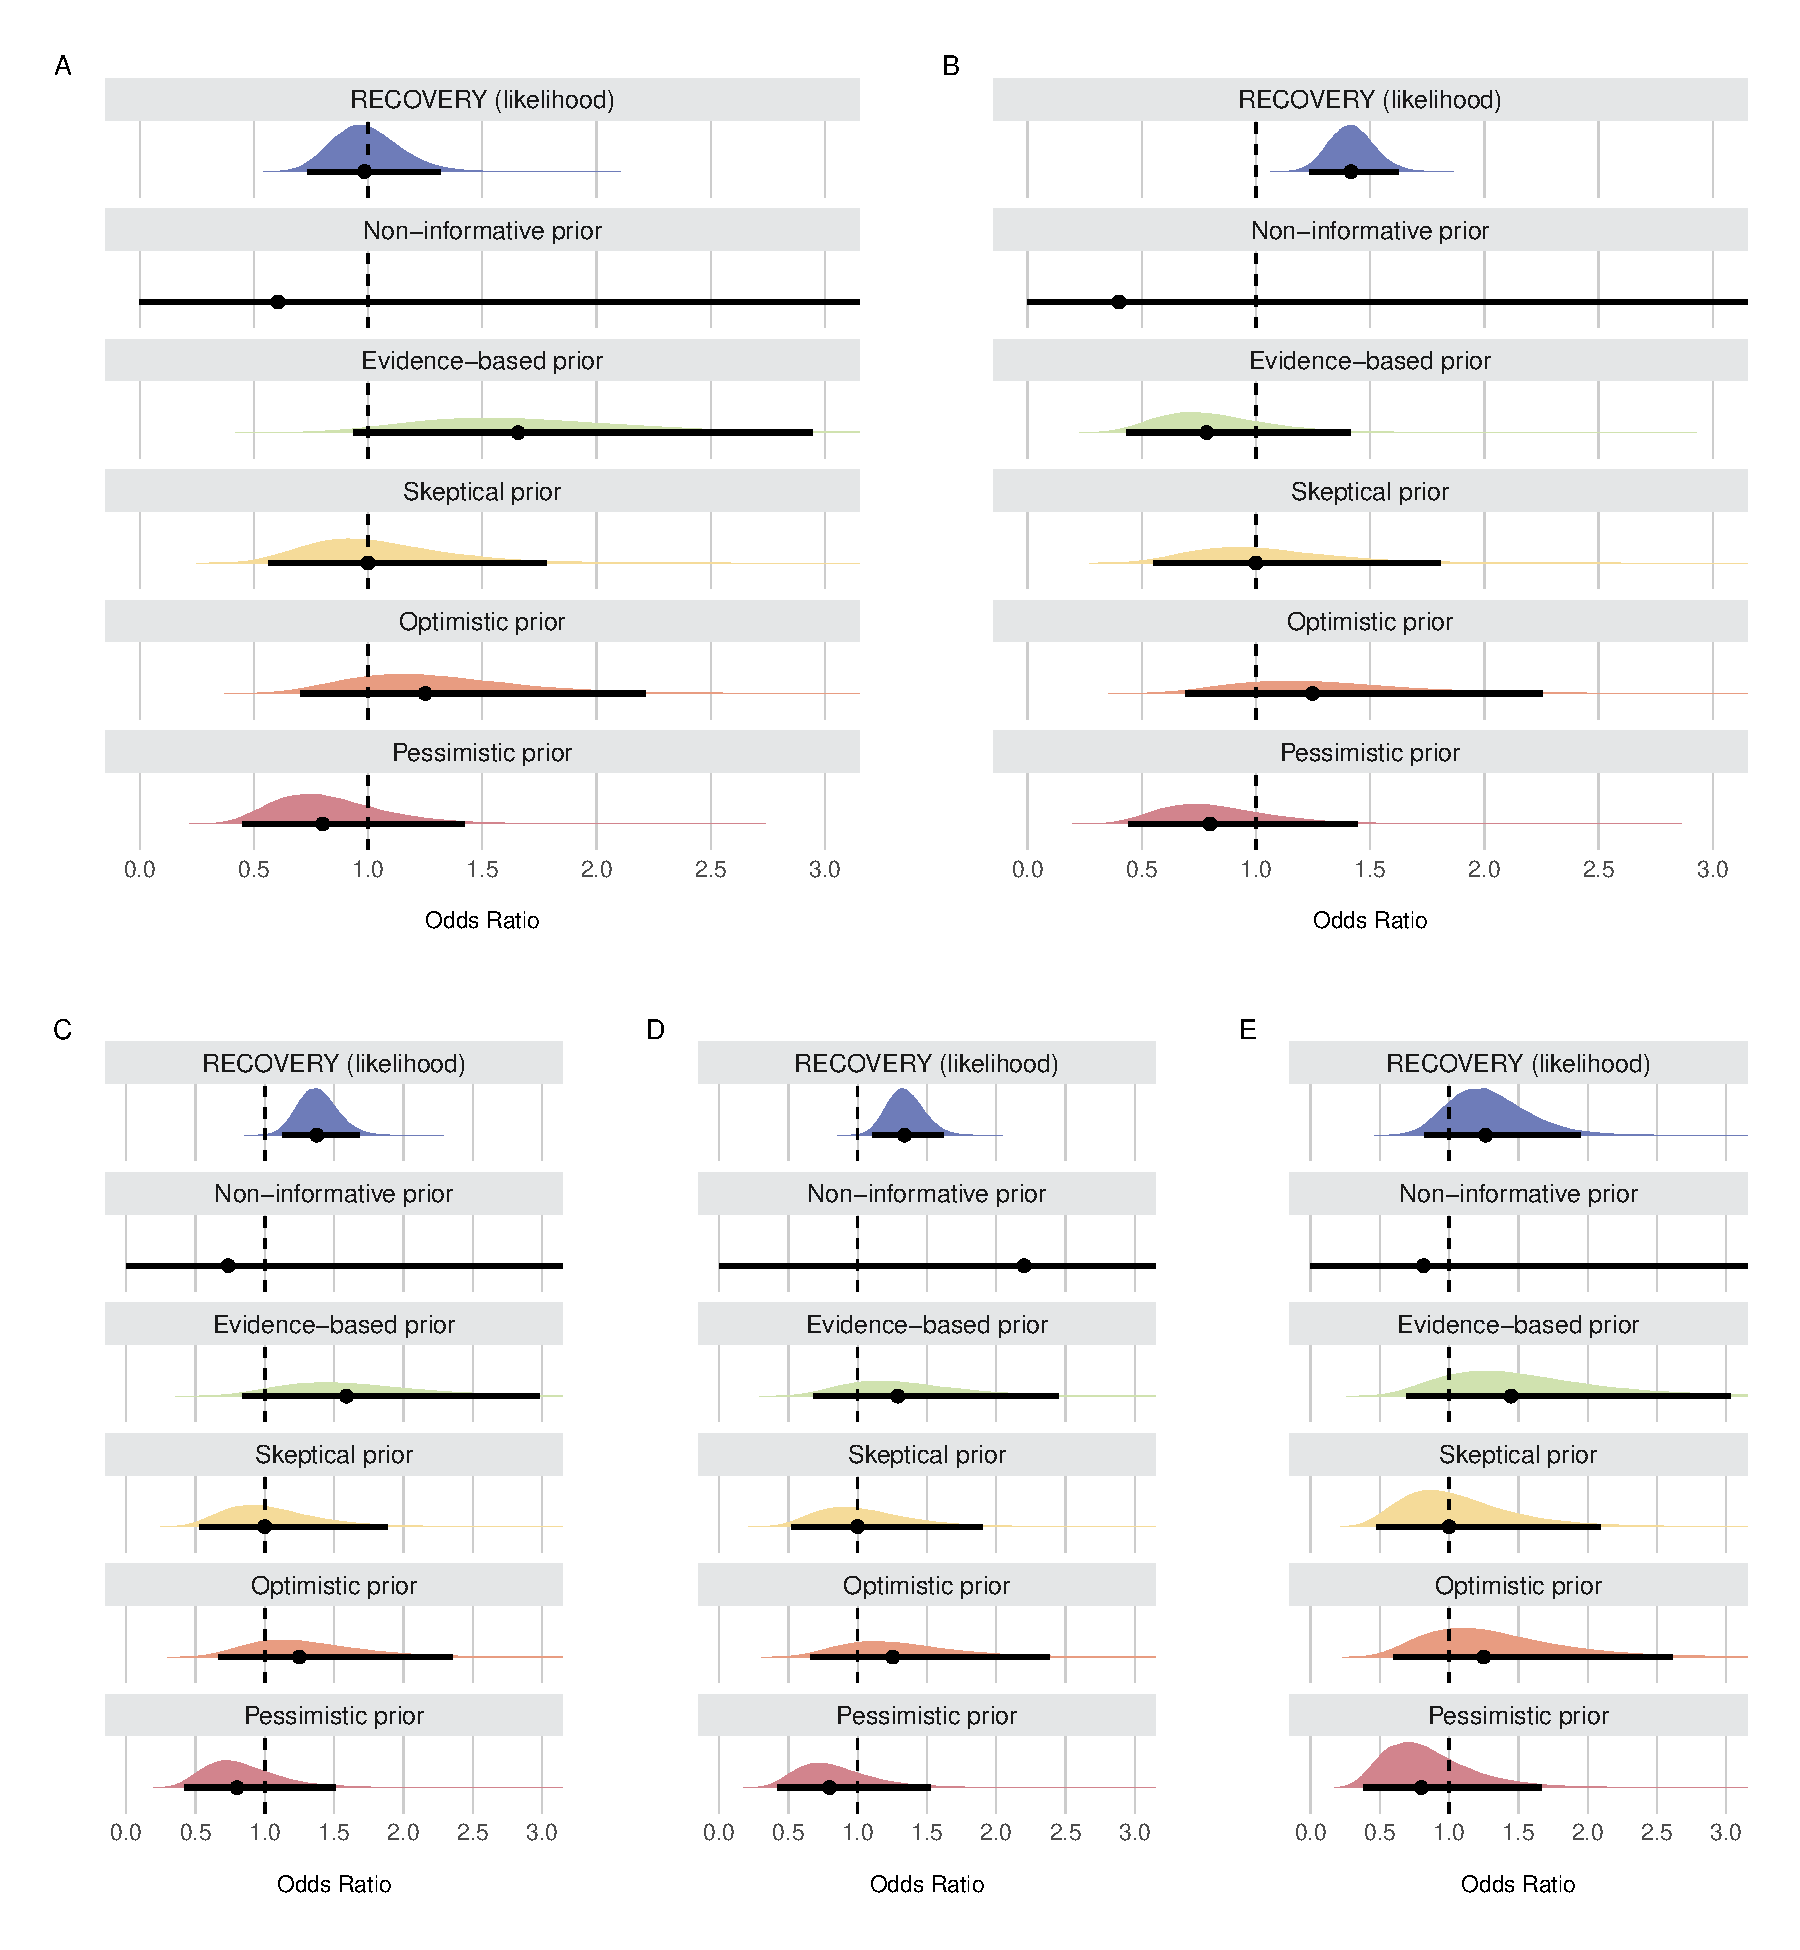
\includegraphics[width=0.95\linewidth]{/Users/arthur/Coding/projects/tocilizumab_reanalysis/final_analyses/output/plots/appendix/SFigure5_discharge_priors_sensitivity} \end{center}

Prior distributions for each subgroup.

Panel A shows results for patients not using corticosteroids; Panel B
shows results for patients using corticosteroids.

Panel C shows results for simple oxygen only; Panel D shows results for
non-invasive ventilation; Panel E shows results for invasive mechanical
ventilation.

Point estimates depict the median and interval bars depict 95th quantile
intervals.

\newpage

\hypertarget{supplementary-figure-6}{%
\subsubsection{Supplementary Figure 6}\label{supplementary-figure-6}}

\begin{center}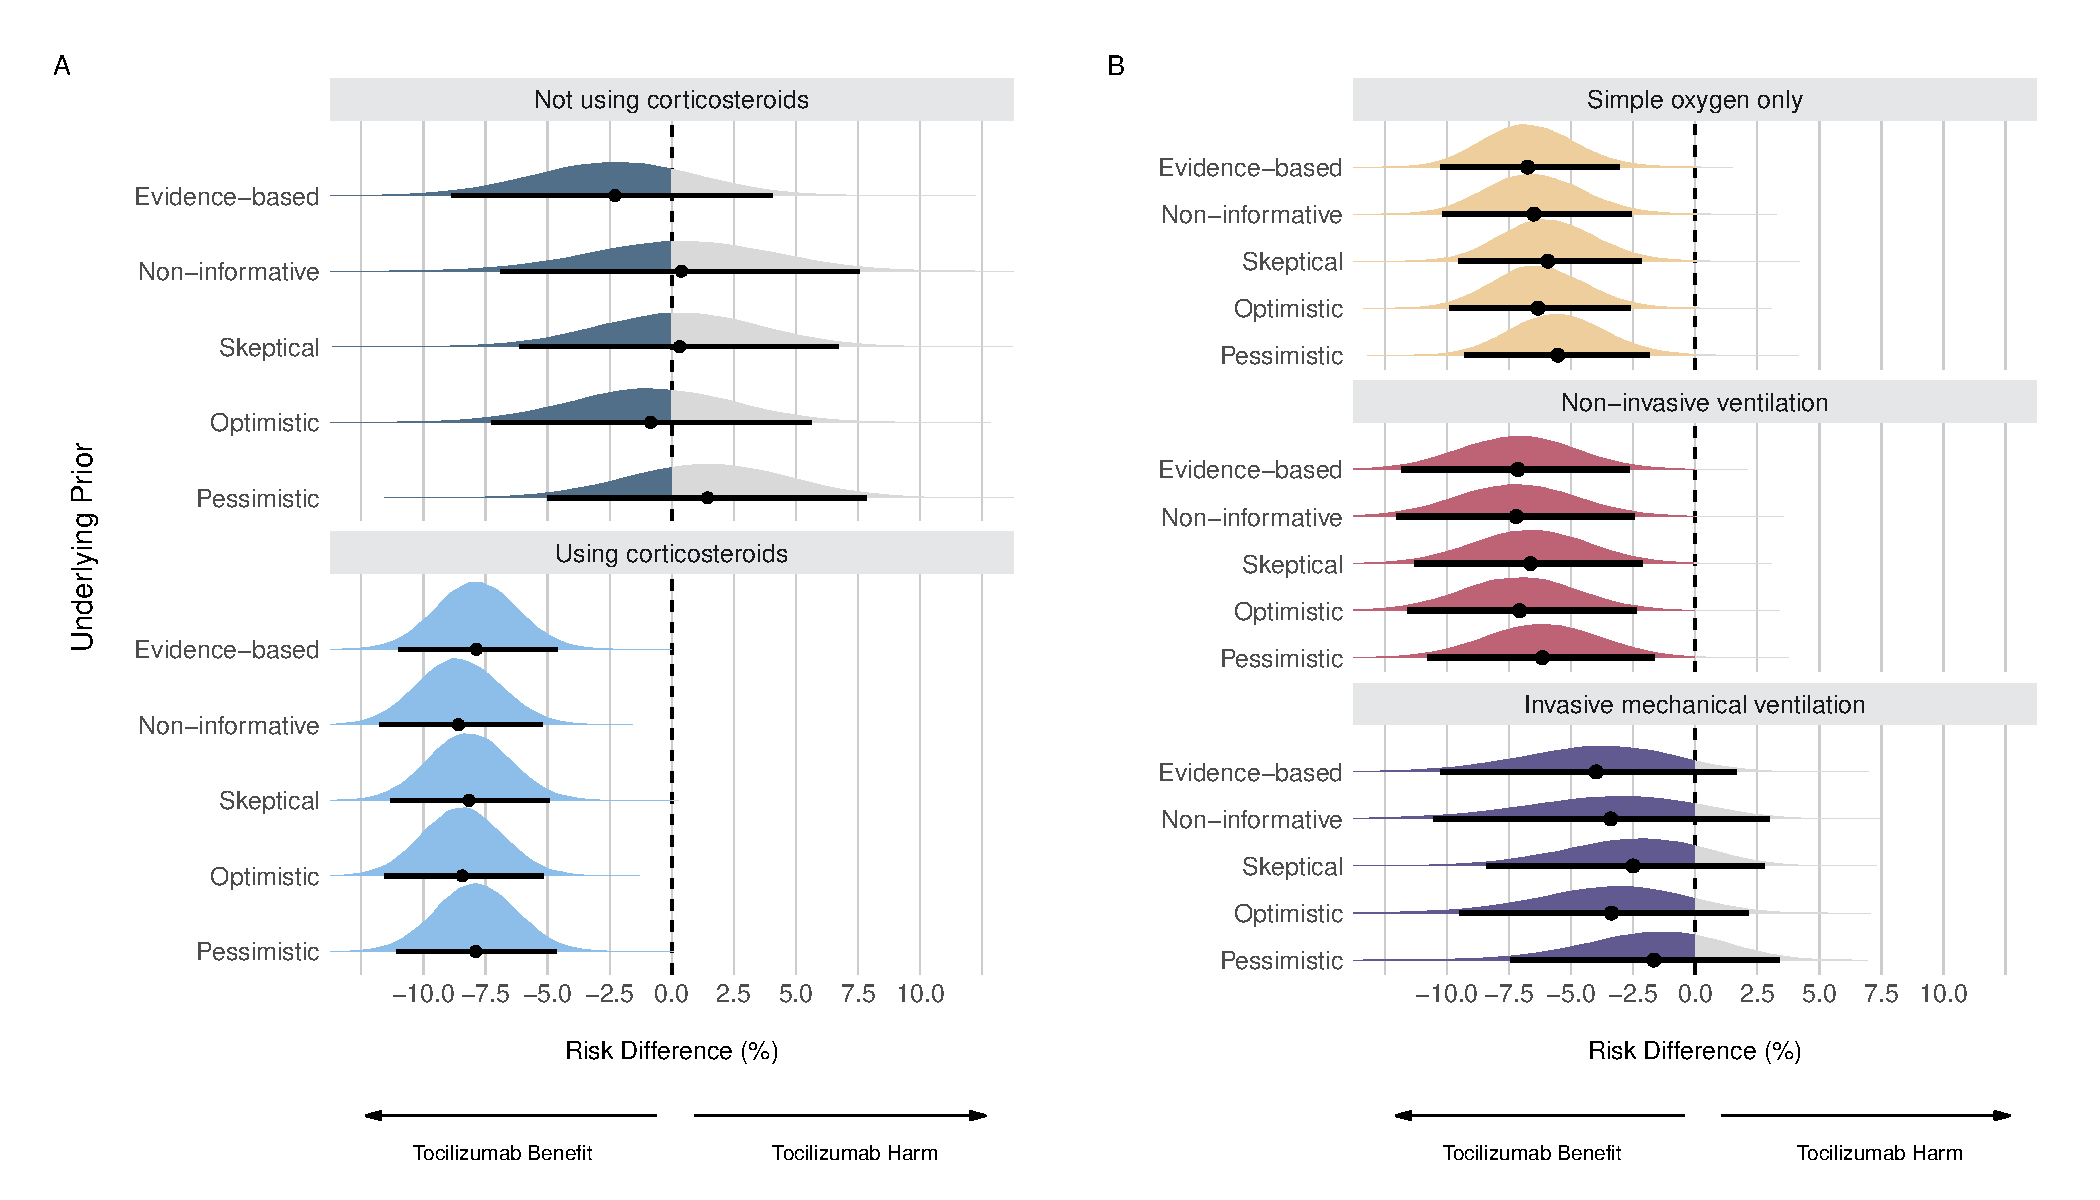
\includegraphics[width=1.1\linewidth]{/Users/arthur/Coding/projects/tocilizumab_reanalysis/final_analyses/output/plots/appendix/SFigure6_discharge_figure3} \end{center}

Posterior distributions from sensitivity analyses using different
priors.

Point estimates depict the median. Interval bars depict the 95\% highest
density intervals.

\newpage

\hypertarget{supplementary-table-7}{%
\subsubsection{Supplementary Table 7}\label{supplementary-table-7}}

\begin{center}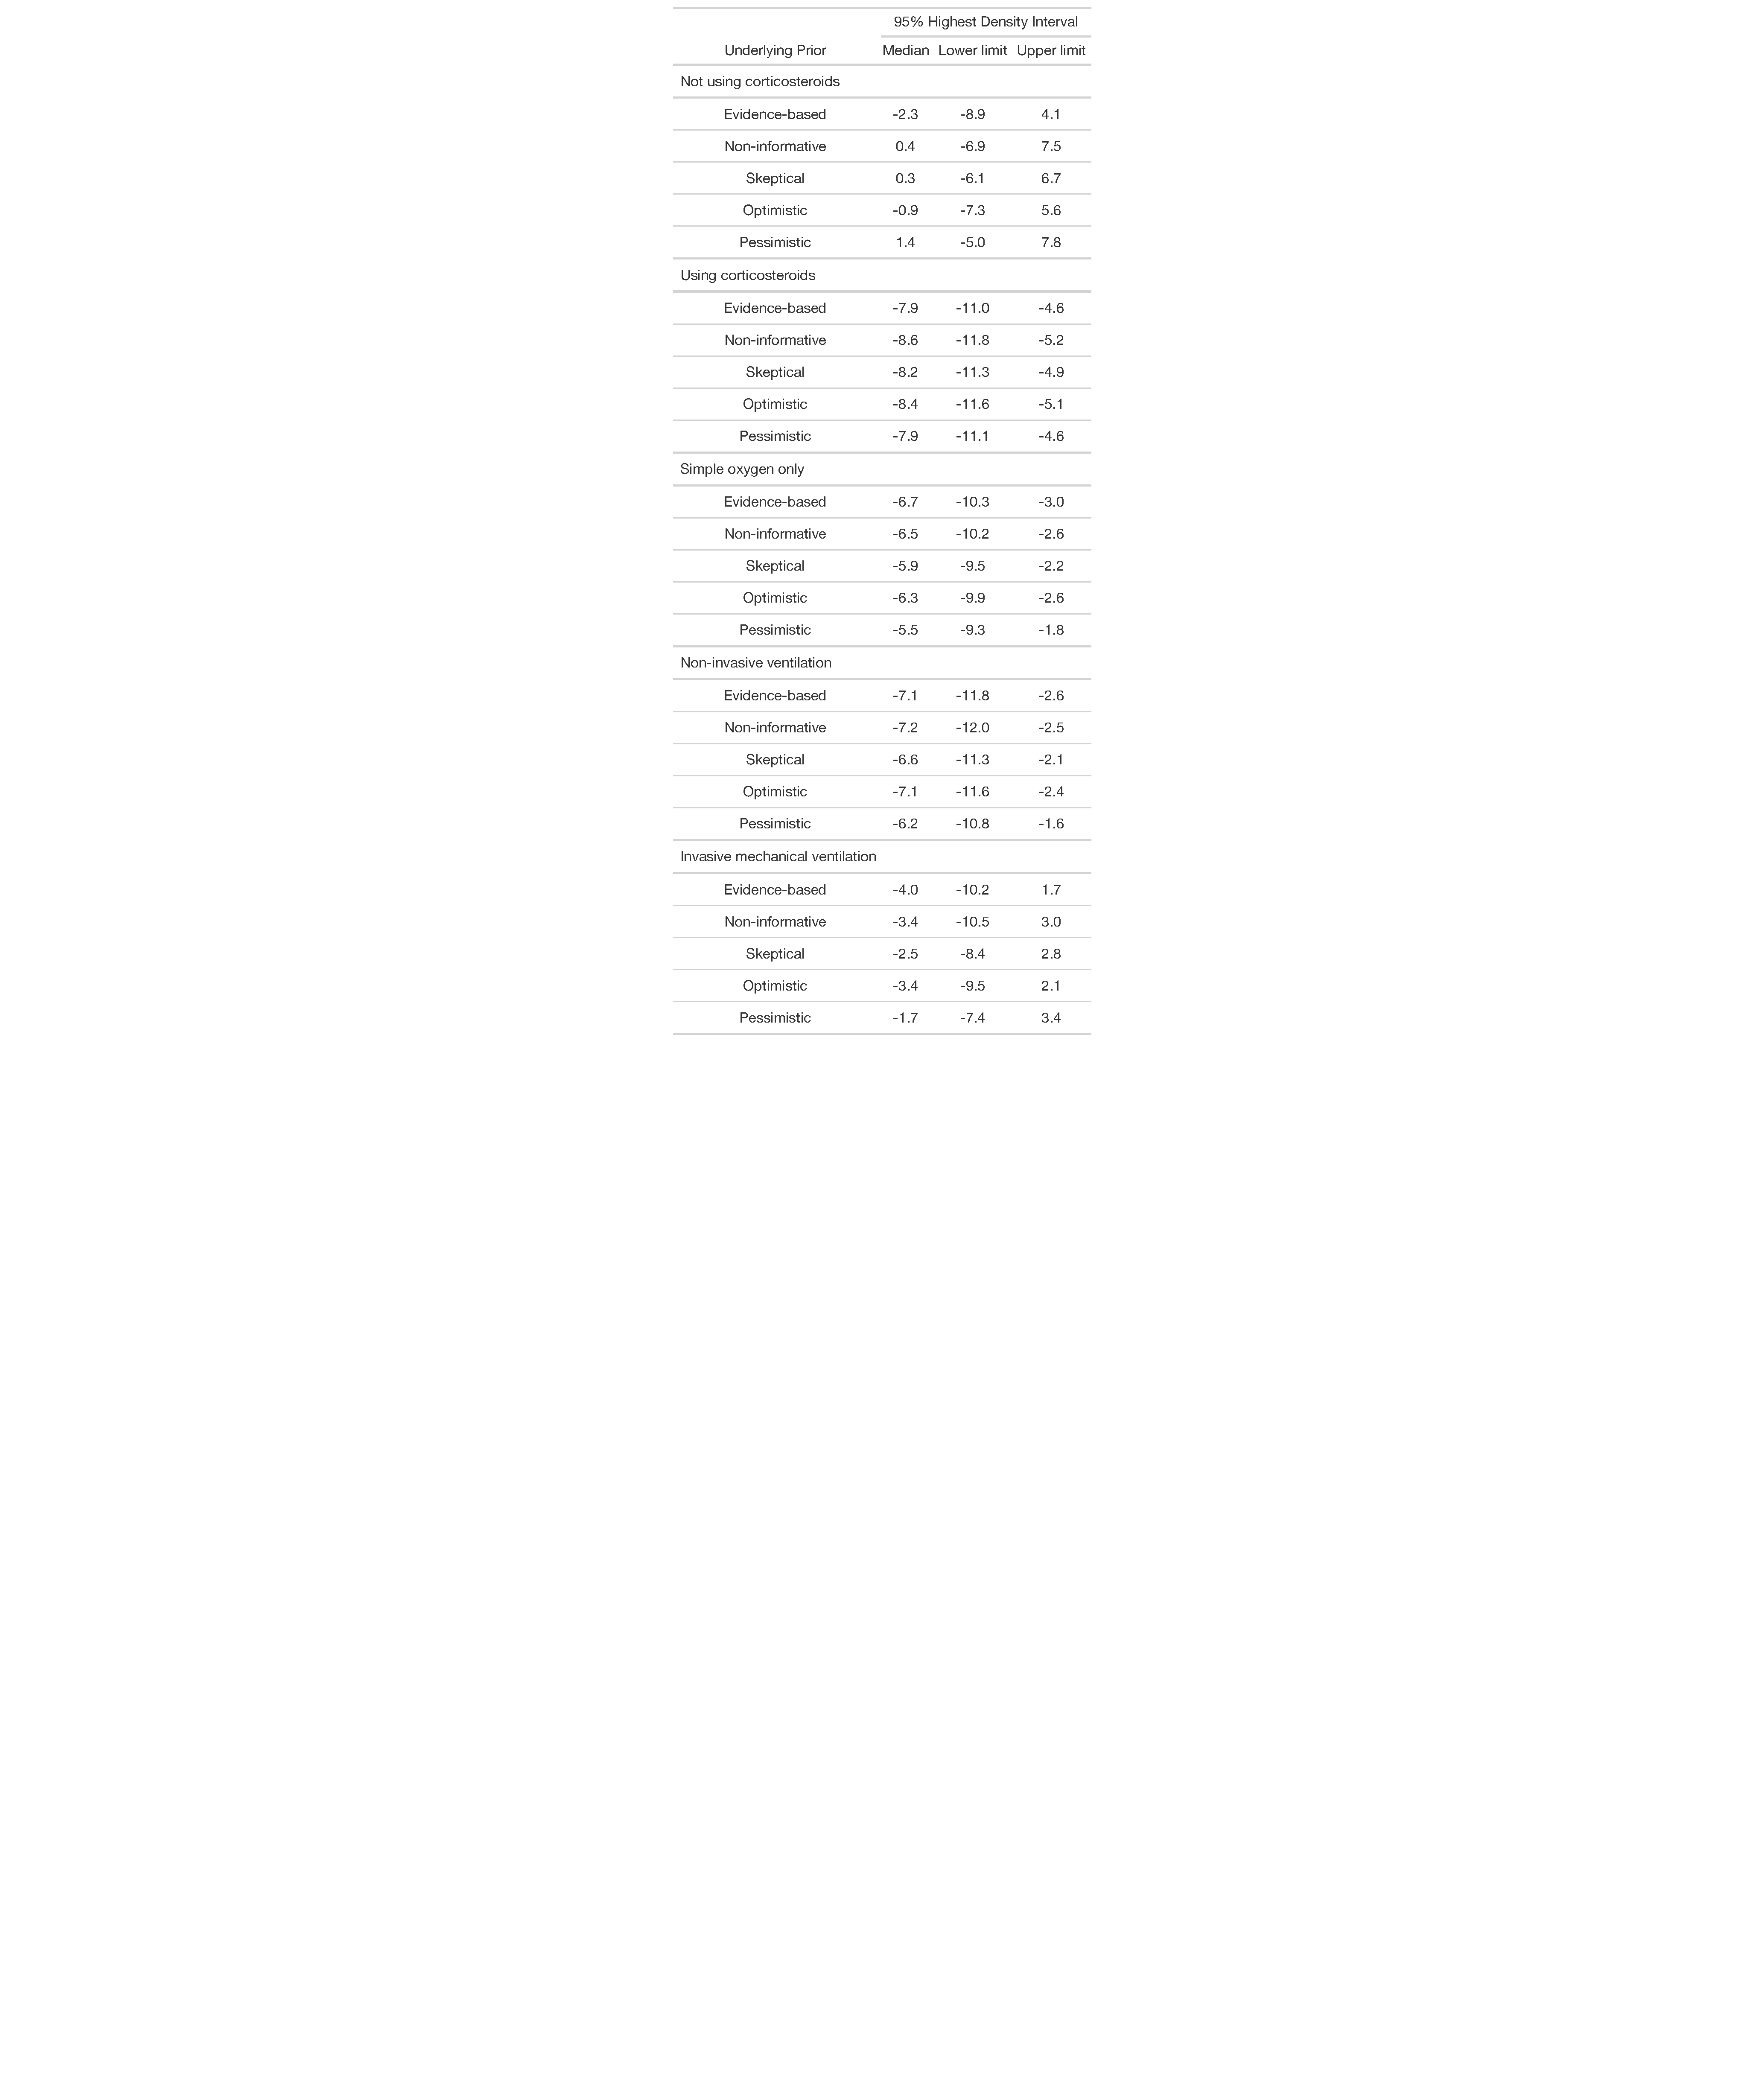
\includegraphics[width=0.5\linewidth]{/Users/arthur/Coding/projects/tocilizumab_reanalysis/final_analyses/output/plots/appendix/STable7_discharge_hdi_figure3} \end{center}

Median and 95\% highest density intervals of posteriors distributions
from sensitivity analyses with different priors. This table complements
Supplementary Figure 6.

\newpage

\hypertarget{supplementary-table-8}{%
\subsubsection{Supplementary Table 8}\label{supplementary-table-8}}

\begin{center}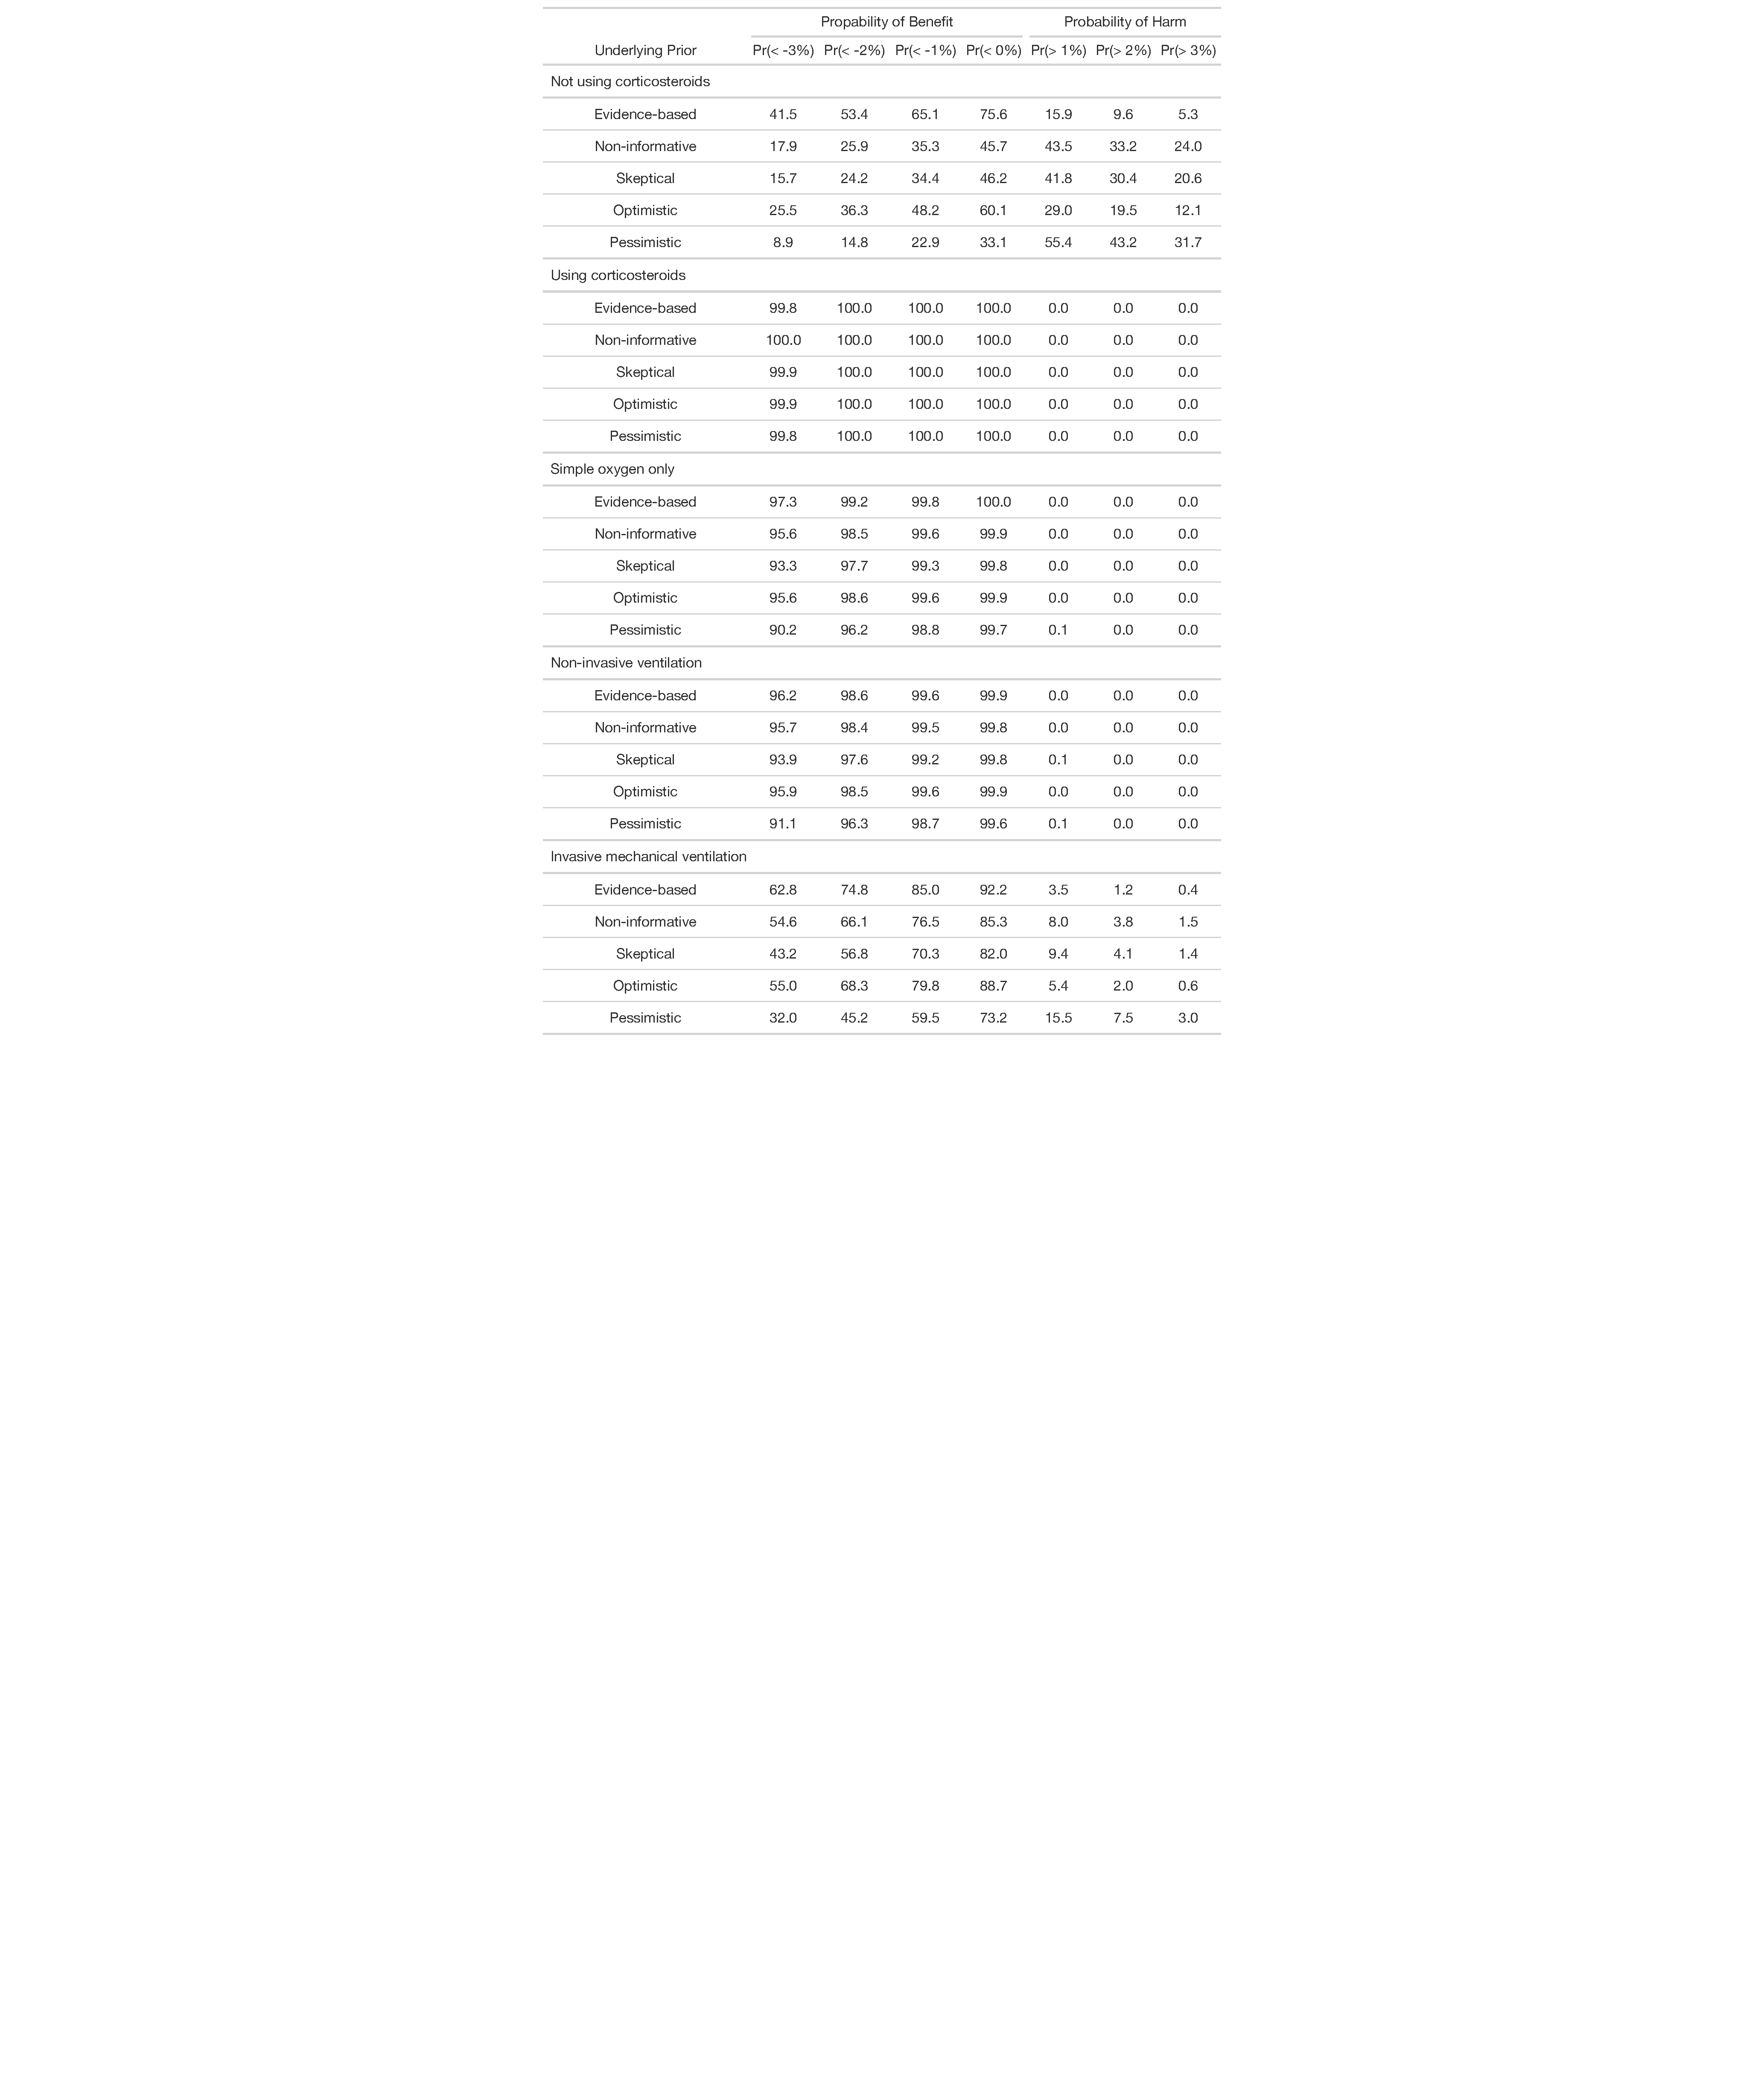
\includegraphics[width=0.8\linewidth]{/Users/arthur/Coding/projects/tocilizumab_reanalysis/final_analyses/output/plots/appendix/STable8_discharge_probabilities_figure3} \end{center}

Posterior probabilities from sensitivity analyses using different
priors. This table complements Supplementary Figure 6.

\newpage

\hypertarget{sensitivity-analyses-using-different-baseline-risks-use-of-corticosteroids}{%
\subsection{Sensitivity analyses using different baseline risks: Use of
corticosteroids}\label{sensitivity-analyses-using-different-baseline-risks-use-of-corticosteroids}}

\hypertarget{supplementary-figure-7}{%
\subsubsection{Supplementary Figure 7}\label{supplementary-figure-7}}

\begin{center}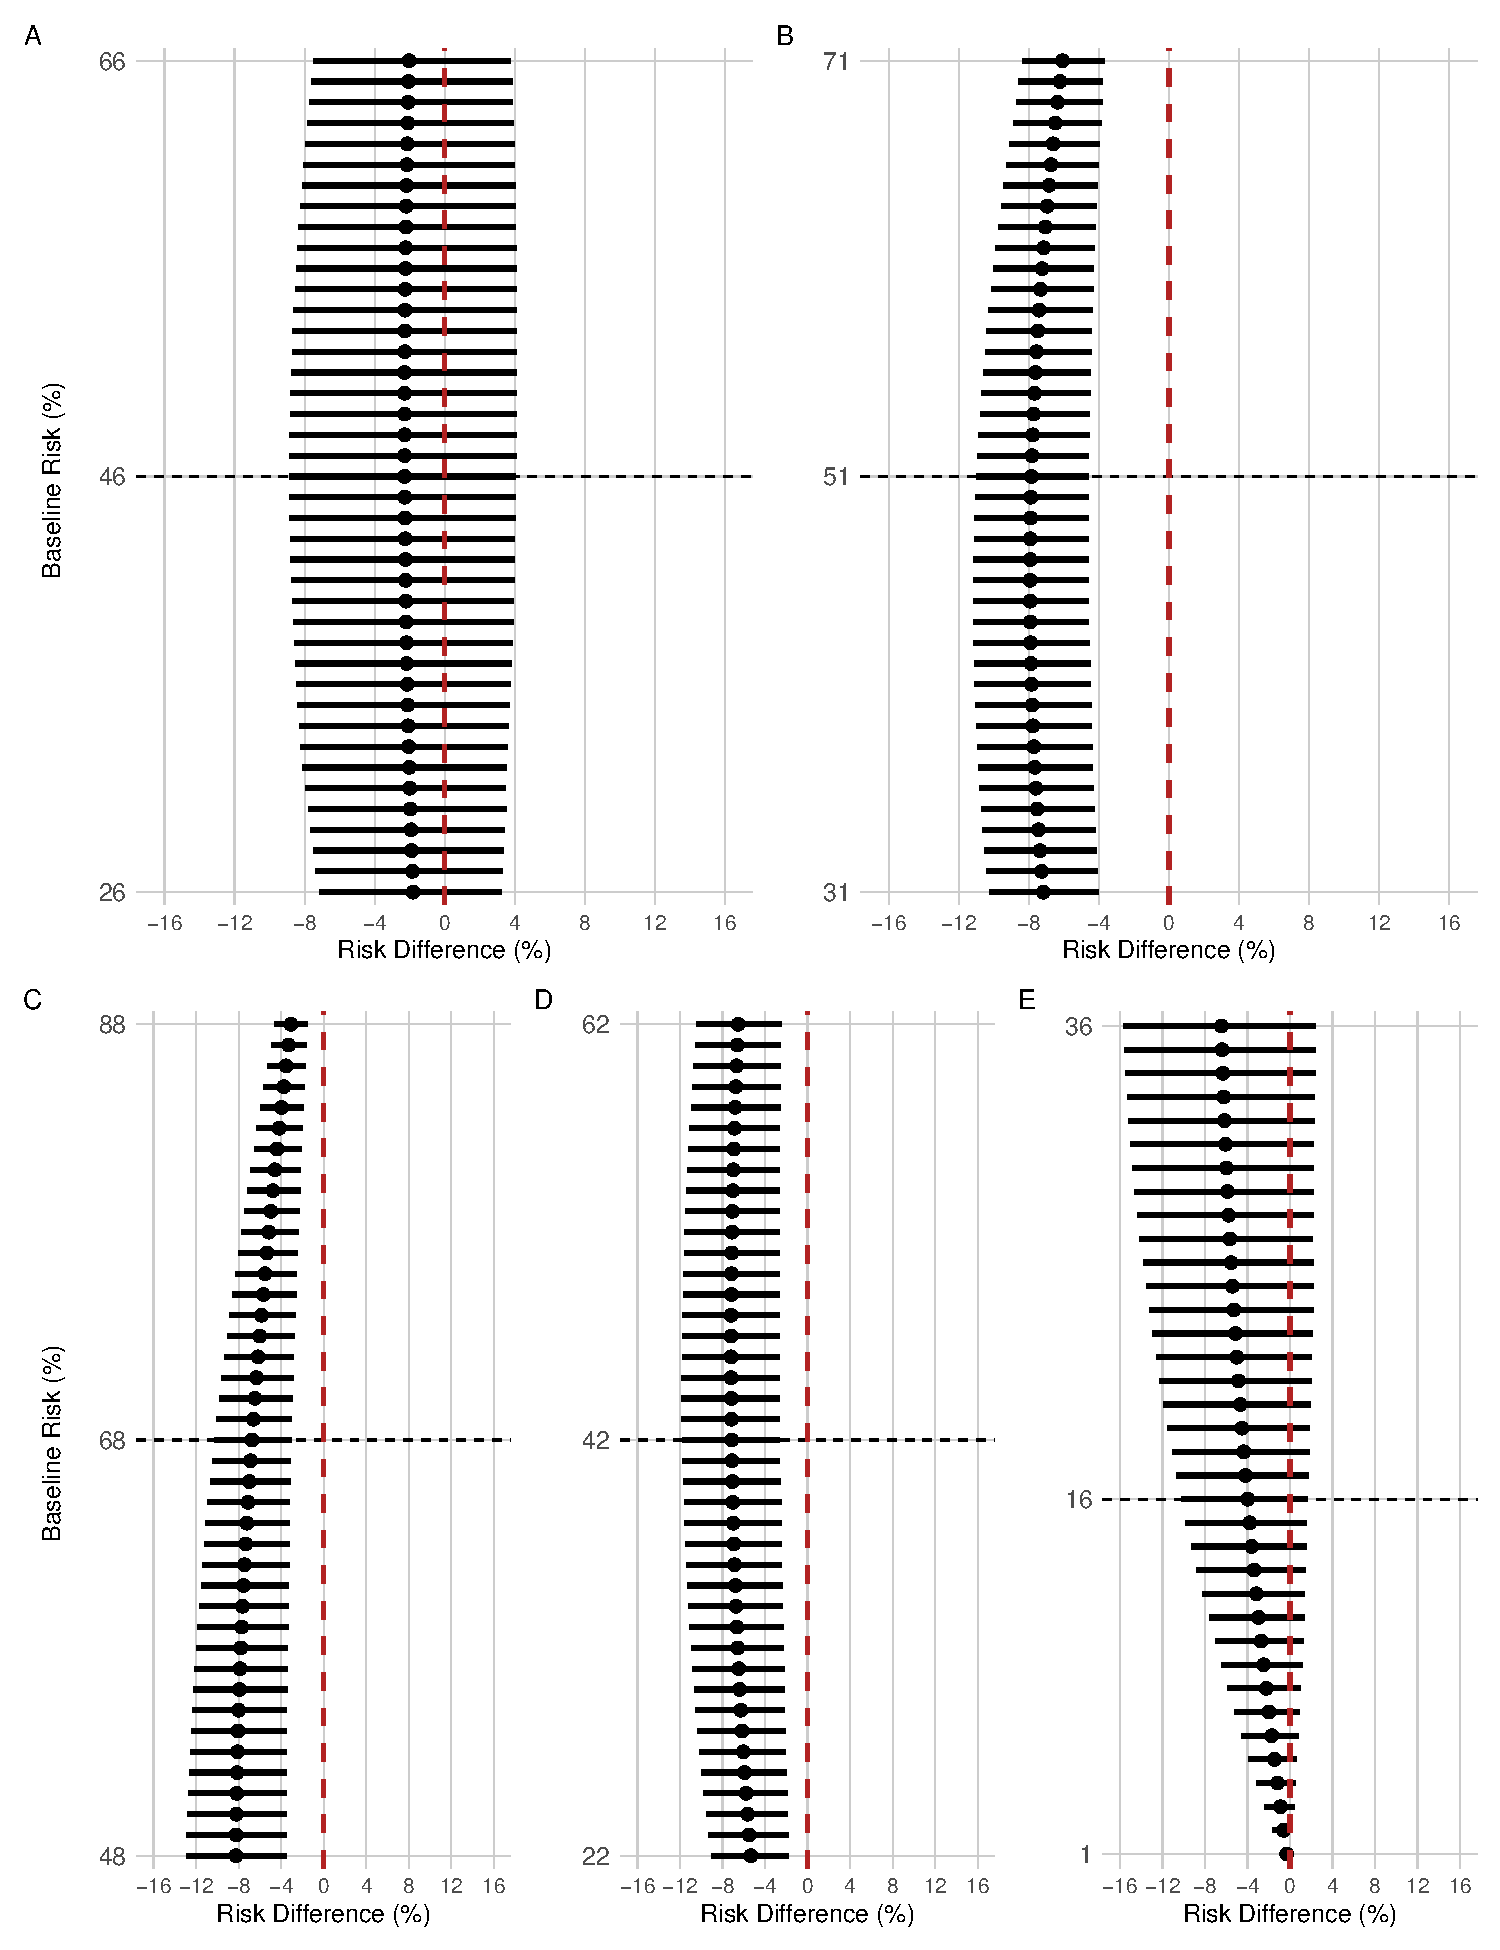
\includegraphics[width=0.7\linewidth]{/Users/arthur/Coding/projects/tocilizumab_reanalysis/final_analyses/output/plots/appendix/SFigure7_discharge_varying_baseline_risk_difference} \end{center}

Posterior distributions from sensitivity analyses using multiple
different baseline risks.

Each line represents posterior distribution for the corresponding
baseline risk. Horizontal black dashed lines represent the respective
baseline risk underlying other analyses (Supplementary Figure 4), i.e.,
risk in the control group in the RECOVERY trial for each subgroup
(Supplementary Table 5). Vertical red dashed line represent 0\% risk
difference. Point estimates depict the median and interval bars depict
95\% highest density intervals.

Panel A shows results for patients not using corticosteroids; Panel B
shows results for patients using corticosteroids. Panel C shows results
for simple oxygen only; Panel D shows results for non-invasive
ventilation; Panel E shows results for invasive mechanical ventilation.

\newpage

\hypertarget{supplementary-figure-8}{%
\subsubsection{Supplementary Figure 8}\label{supplementary-figure-8}}

\begin{center}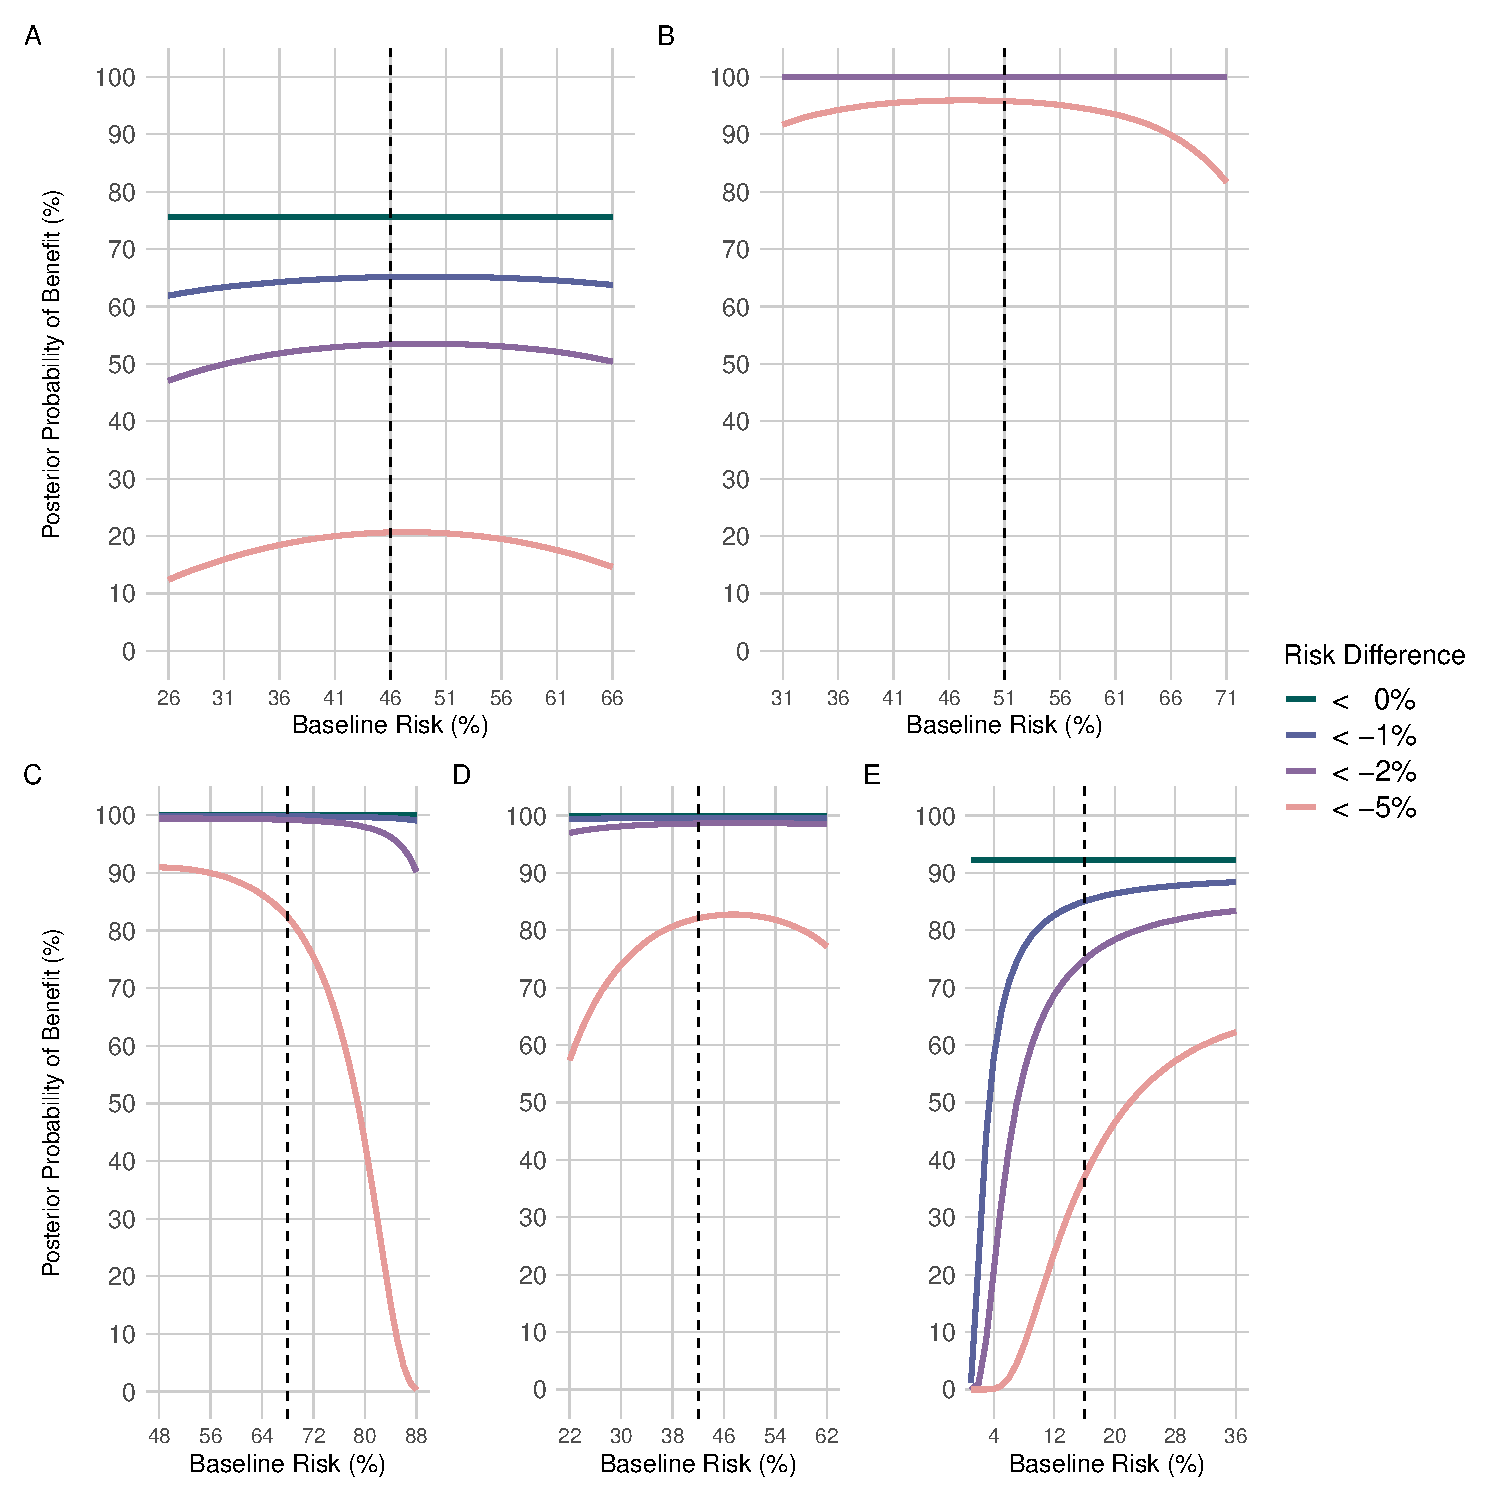
\includegraphics[width=1\linewidth]{/Users/arthur/Coding/projects/tocilizumab_reanalysis/final_analyses/output/plots/appendix/SFigure8_discharge_figure4} \end{center}

Posterior probabilities from sensitivity analyses using multiple
different baseline risks.

Each line represents the posterior probability of benefit for a specific
cutoff, such as risk difference lower to 0\%, 1\%, 2\% and 5\%. Vertical
black dashed lines represent the respective baseline risk underlying
other analyses (Supplementary Figure 4), i.e., risk in the control group
in the RECOVERY trial for each subgroup (Supplementary Table 5).

Panel A shows results for patients not using corticosteroids; Panel B
shows results for patients using corticosteroids. Panel C shows results
for simple oxygen only; Panel D shows results for non-invasive
ventilation; Panel E shows results for invasive mechanical ventilation.

\end{document}
